% lecture9_ro.tex -- GENERATED by build_L9.py from L9_numbers.json; do not edit by hand.
\documentclass[10pt,aspectratio=169,t]{beamer}
% =============================================================================
% nn_preamble.tex -- shared Beamer preamble of Neural Networks and Deep Learning (NN)
% Used by every lecture: lectures/Lk/lecturek.tex does
%   \documentclass[10pt,aspectratio=169,t]{beamer}
%   % =============================================================================
% nn_preamble.tex -- shared Beamer preamble of Neural Networks and Deep Learning (NN)
% Used by every lecture: lectures/Lk/lecturek.tex does
%   \documentclass[10pt,aspectratio=169,t]{beamer}
%   % =============================================================================
% nn_preamble.tex -- shared Beamer preamble of Neural Networks and Deep Learning (NN)
% Used by every lecture: lectures/Lk/lecturek.tex does
%   \documentclass[10pt,aspectratio=169,t]{beamer}
%   \input{../common/nn_preamble}
%   \nnlecture{k}{Lecture title}
% Logos live in lectures/common/logos/, charts in lectures/Lk/charts/.
% Do NOT add \hfuzz / \vfuzz / \hbadness here: overfull boxes must be fixed, not hidden.
% =============================================================================

\usetheme{default}
\setbeamersize{text margin left=7mm, text margin right=7mm}

% ---------------------------------------------------------------- packages
\usepackage[utf8]{inputenc}
\usepackage[T1]{fontenc}
\usepackage{lmodern}
\usepackage{amsmath, amssymb}
\usepackage{mathtools}
\usepackage{bm}
\usepackage{tikz}
\usetikzlibrary{arrows.meta, positioning, calc, shapes.misc}
\usepackage{booktabs}
\usepackage{array}
\usepackage{graphicx}
\usepackage{colortbl}
\usepackage{xcolor}
\usepackage{multicol}
\hypersetup{colorlinks=true, linkcolor=MainBlue, urlcolor=MainBlue, citecolor=MainBlue}
\graphicspath{{../common/logos/}}   % charts are included with their language folder: charts/en/, charts/ro/

% ---------------------------------------------------------------- colours
\definecolor{MainBlue}{RGB}{26, 58, 110}
\definecolor{IDAred}{RGB}{205, 0, 0}
\definecolor{DarkGray}{RGB}{51, 51, 51}
\definecolor{FooterGray}{RGB}{100, 100, 100}
\definecolor{BlockGray}{RGB}{236, 238, 242}
\definecolor{KeynoteGray}{RGB}{218, 218, 218}
\definecolor{Crimson}{RGB}{190, 40, 50}
\definecolor{Forest}{RGB}{30, 110, 50}
\definecolor{Bitter}{RGB}{214, 150, 20}
% chart palette (same hex values and order as lectures/common/nn_plot.py SERIES)
\definecolor{Ser1}{HTML}{2A78D6}
\definecolor{Ser2}{HTML}{EB6834}
\definecolor{Ser3}{HTML}{1BAF7A}
\definecolor{Ser4}{HTML}{EDA100}
\definecolor{Ser5}{HTML}{E87BA4}
\definecolor{Ser6}{HTML}{008300}
\definecolor{Ser7}{HTML}{6250D6}
\definecolor{Ser8}{HTML}{E34948}

\setbeamertemplate{background}{%
  \begin{tikzpicture}[remember picture, overlay]
    \shade[shading=axis, shading angle=315, top color=white, bottom color=KeynoteGray]
      (current page.south west) rectangle (current page.north east);
  \end{tikzpicture}}
\setbeamercolor{background canvas}{bg=}
\setbeamercolor{structure}{fg=MainBlue}
\setbeamercolor{normal text}{fg=DarkGray}
\setbeamercolor{title}{fg=IDAred}
\setbeamercolor{frametitle}{fg=IDAred, bg=}
\setbeamercolor{block title}{bg=MainBlue, fg=white}
\setbeamercolor{block body}{bg=BlockGray, fg=DarkGray}
\setbeamercolor{block title alerted}{bg=Crimson, fg=white}
\setbeamercolor{block body alerted}{bg=Crimson!7, fg=DarkGray}
\setbeamercolor{block title example}{bg=Forest, fg=white}
\setbeamercolor{block body example}{bg=Forest!7, fg=DarkGray}
\setbeamercolor{item}{fg=MainBlue}
\setbeamerfont{frametitle}{size=\large, series=\bfseries}
\setbeamerfont{block title}{size=\small, series=\bfseries}
\setbeamertemplate{blocks}[rounded][shadow=false]
\setbeamertemplate{itemize item}{\color{MainBlue}$\boxdot$}
\setbeamertemplate{itemize subitem}{\color{MainBlue}\scriptsize$\blacktriangleright$}
% compact two-level lists: level 1 = main point, level 2 = details (no text outside bullets)
\setbeamerfont{itemize/enumerate subbody}{size=\footnotesize}
\setlength{\leftmargini}{1.1em}
\setlength{\leftmarginii}{1.1em}
\setbeamertemplate{itemize/enumerate body begin}{\setlength{\topsep}{0pt}\setlength{\partopsep}{0pt}\setlength{\parskip}{0pt}}
\setbeamertemplate{itemize/enumerate subbody begin}{\setlength{\topsep}{0pt}\setlength{\partopsep}{0pt}\setlength{\itemsep}{0pt}\vspace{-0.4ex}}

\setbeamertemplate{enumerate item}{\color{MainBlue}\insertenumlabel.}
\setlength{\leftmargini}{1.3em}
\setlength{\leftmarginii}{1.2em}
\setbeamertemplate{navigation symbols}{}
\setbeamertemplate{section in toc}{\color{MainBlue}$\blacktriangleright$~\inserttocsection}
\setbeamertemplate{caption}{\raggedright\insertcaption\par}
% frame subtitle = precise citation line under the claim title (Weron style)
\setbeamerfont{framesubtitle}{size=\footnotesize}
\setbeamercolor{framesubtitle}{fg=FooterGray}
% outline that reappears at every section with the current section highlighted
\setbeamertemplate{section in toc shaded}[default][35]
\setbeamertemplate{subsection in toc shaded}[default][35]
\setbeamertemplate{subsection in toc}{\leavevmode\leftskip=2.2em\color{DarkGray}\small\inserttocsubsection\par}
\AtBeginSection[]{{\begin{frame}{\txtoutline}\vspace{2mm}\small
  \tableofcontents[currentsection,hideothersubsections]\end{frame}}}

% ---------------------------------------------------------------- head and foot
\setbeamertemplate{headline}{%
  \vskip10pt%
  \hbox to \paperwidth{\hskip0.5cm%
    {\small\color{FooterGray}\renewcommand{\hyperlink}[2]{##2}\insertsectionhead}%
    \hfill\textcolor{FooterGray}{\small\insertframenumber}\hskip0.5cm}%
  \vskip4pt{\color{FooterGray}\hrule height 0.4pt}}
% footer as in the other courses (MFM, SFM): course name on the left, small sparkline on the right
\setbeamertemplate{footline}{%
  {\color{FooterGray}\hrule height 0.4pt}\vskip4pt%
  \hbox to \paperwidth{\hskip0.5cm%
    \textcolor{FooterGray}{\small\txtcourse}%
    \hfill\raisebox{-0.1em}{\begin{tikzpicture}[x=0.08em, y=0.08em, line width=0.4pt]
      \draw[FooterGray] (0,3) -- (1,4) -- (2,3.5) -- (3,5) -- (4,4) -- (5,6) -- (6,5.5) -- (7,4) -- (8,5) -- (9,7) -- (10,6) -- (11,5) -- (12,6.5) -- (13,8) -- (14,7) -- (15,6) -- (16,7.5) -- (17,9) -- (18,8) -- (19,7) -- (20,8.5) -- (21,10) -- (22,9) -- (23,8) -- (24,9.5);
    \end{tikzpicture}}\hskip0.5cm}%
  \vskip6pt}

% ---------------------------------------------------------------- title page
\defbeamertemplate*{title page}{nn}[1][]{%
  \vspace{0.15cm}
  \begin{center}
    \href{https://www.ase.ro}{
\includegraphics[height=0.9cm]{ase_logo.png}}\hspace{0.3cm}%
    \href{https://ipe.ro/new}{
\includegraphics[height=0.9cm]{acad_logo.png}}\hspace{0.3cm}%
    \href{https://theida.net}{
\includegraphics[height=0.9cm]{ida_logo.png}}\hspace{0.3cm}%
    \href{https://blockchain-research-center.com}{
\includegraphics[height=0.9cm]{brc_logo.png}}\hspace{0.3cm}%
    \href{https://www.ai4efin.ase.ro}{
\includegraphics[height=0.9cm]{ai4efin_logo.png}}\hspace{0.3cm}%
    \href{https://www.digital-finance-msca.com}{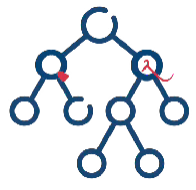
\includegraphics[height=0.9cm]{msca_logo.png}}%
  \end{center}
  \vspace{0.45cm}
  \begin{center}
    \begin{minipage}{0.1\textwidth}\centering
      \href{https://quantlet.com}{
\includegraphics[height=0.9cm]{ql_logo.png}}\end{minipage}%
    \begin{minipage}{0.78\textwidth}\centering
      {\Large\bfseries\usebeamercolor[fg]{title}\inserttitle}\par\vspace{0.25cm}
      {\large\usebeamercolor[fg]{title}\insertsubtitle}\end{minipage}%
    \begin{minipage}{0.1\textwidth}\centering
      \href{https://quantinar.com}{
\includegraphics[height=0.9cm]{qr_logo.png}}\end{minipage}
  \end{center}
  \vfill
  \hspace{0.4cm}{\bfseries\insertauthor}\par\vspace{0.12cm}
  \hspace{0.4cm}\begin{minipage}[t]{0.92\textwidth}\raggedright\footnotesize\insertinstitute\end{minipage}
  \par\vspace{0.4cm}}

% ---------------------------------------------------------------- lecture metadata
\newcommand{\nnshort}{}
\newcommand{\nnnb}{notebooks}
\newcommand{\nnrepo}{https://github.com/danpele/NEURAL_BIZ/tree/main}
% language-dependent labels (English default; \nnromanian switches to Romanian, call it before \nnlecture)
\newcommand{\txtcourse}{Neural Networks and Deep Learning}
\newcommand{\txtlecture}{Lecture}
\newcommand{\txtoutline}{Outline}
\newcommand{\txtintuition}{In one sentence:}
\newcommand{\txtjob}{In practice:}
\newcommand{\txttry}{Experiment yourself:}
\newcommand{\txtwhere}{where}
\newcommand{\txtsim}{SIMULATED DATA (teaching illustration)}
\newcommand{\txtnbsuffix}{}
\newcommand{\txtinstitute}{Bucharest University of Economic Studies (ASE), Department of Statistics and Econometrics\\
    Romanian Academy, Institute for Economic Forecasting (IPE)\\
    IDA Institute Digital Assets \textbullet\ AI4EFin \textbullet\ MSCA Digital Finance}
\newcommand{\nnromanian}{%
  \renewcommand{\txtcourse}{Rețele neuronale și deep learning}%
  \renewcommand{\txtlecture}{Cursul}%
  \renewcommand{\txtoutline}{Cuprins}%
  \renewcommand{\txtintuition}{Pe scurt:}%
  \renewcommand{\txtjob}{În practică:}%
  \renewcommand{\txttry}{Exercițiu practic:}%
  \renewcommand{\txtwhere}{unde}%
  \renewcommand{\txtsim}{DATE SIMULATE (doar pentru ilustrare)}%
  \renewcommand{\txtnbsuffix}{\string_ro}%
  \renewcommand{\txtinstitute}{Academia de Studii Economice din București (ASE), Departamentul de Statistică și Econometrie\\
    Academia Română, Institutul de Prognoză Economică (IPE)\\
    IDA Institute Digital Assets \textbullet\ AI4EFin \textbullet\ MSCA Digital Finance}}
\newcommand{\nnlecture}[2]{%
  \renewcommand{\nnshort}{\txtlecture\ #1}%
  \renewcommand{\nnnb}{notebooks/L#1\string_notebook\txtnbsuffix.ipynb}%
  \title[NN]{\txtcourse}%
  \subtitle{\txtlecture\ #1: #2}%
  \author{Prof.\ dr.\ Daniel Traian PELE}%
  \institute{\txtinstitute}%
  \date{}}

% ---------------------------------------------------------------- teaching blocks (one message per frame)
% \intuition{one plain sentence}  ->  formula with every symbol defined  ->  real-data example  ->  \manager{one line}
\newcommand{\intuition}[1]{\begin{itemize}\item {\color{MainBlue}\textbf{\txtintuition}}~#1\end{itemize}\vspace{0.6mm}}
\newcommand{\manager}[1]{\colorbox{Forest!10}{\parbox{\dimexpr\linewidth-2\fboxsep\relax}{\footnotesize
  \begin{itemize}\setlength{\itemsep}{0pt}\item \textbf{\color{Forest}\txtjob}~#1\end{itemize}}}}
% Experiment yourself: pointer to the matching notebook section
\newcommand{\tryit}[1]{{\scriptsize\href{\nnrepo/\nnnb}{%
  \raisebox{-0.15em}{
\includegraphics[height=0.85em]{ql_logo.png}}\,\textbf{\txttry}~\color{MainBlue}#1}}}
% bottom row: manager line (left) + experiment pointer (right), pinned to the bottom of the frame
\newcommand{\bottomrow}[2]{\par\vfill\noindent\begin{minipage}[b]{0.72\linewidth}#1\end{minipage}\hfill
  \begin{minipage}[b]{0.26\linewidth}\raggedleft #2\end{minipage}\par\vspace{0.5mm}}
\newcommand{\where}[1]{{\footnotesize\textbf{\txtwhere}~#1\par}}

% ---------------------------------------------------------------- helpers
% chart source line under a figure: \chartsource{Source ...; period ...}
\newcommand{\chartsource}[1]{\par\vspace{1pt}{\scriptsize\color{FooterGray}#1\par}}
% link to code: \quantlet{label}{path inside the repo}
\newcommand{\quantlet}[2]{\par\vspace{1pt}\hfill\href{\nnrepo/#2}{%
  \raisebox{-0.15em}{
\includegraphics[height=0.75em]{ql_logo.png}}\textcolor{MainBlue}{\scriptsize\ #1}}}
% inline Quantlet link for the bottom-right corner of a frame: \qlink{label}{path inside the repo}
\newcommand{\qlink}[2]{{\scriptsize\href{\nnrepo/#2}{\raisebox{-0.15em}{
\includegraphics[height=0.85em]{ql_logo.png}}\,\textcolor{MainBlue}{#1}}}}
\newcommand{\simlabel}{\colorbox{Crimson!12}{\scriptsize\bfseries\color{Crimson}\txtsim}}
\newcommand{\E}{\mathbb{E}}
\newcommand{\Var}{\operatorname{Var}}
\newcommand{\Cov}{\operatorname{Cov}}
\newcommand{\Corr}{\operatorname{Corr}}
\newcommand{\asinh}{\operatorname{asinh}}
\newcommand{\iid}{\overset{\text{i.i.d.}}{\sim}}
\newcommand{\EUR}{EUR}
% deep-learning notation (Bishop & Bishop, 2024): vectors bold lower case, matrices bold upper case
\newcommand{\R}{\mathbb{R}}
\newcommand{\vx}{\mathbf{x}}
\newcommand{\vy}{\mathbf{y}}
\newcommand{\vz}{\mathbf{z}}
\newcommand{\vh}{\mathbf{h}}
\newcommand{\vw}{\mathbf{w}}
\newcommand{\vb}{\mathbf{b}}
\newcommand{\mW}{\mathbf{W}}
\newcommand{\mX}{\mathbf{X}}
\newcommand{\btheta}{\boldsymbol{\theta}}
\newcommand{\loss}{\mathcal{L}}
\newcommand{\dataset}{\mathcal{D}}
\DeclareMathOperator*{\argmin}{arg\,min}
\DeclareMathOperator*{\argmax}{arg\,max}
\DeclareMathOperator{\softmax}{softmax}
\DeclareMathOperator{\ReLU}{ReLU}
\DeclareMathOperator{\sigm}{\sigma}

%   \nnlecture{k}{Lecture title}
% Logos live in lectures/common/logos/, charts in lectures/Lk/charts/.
% Do NOT add \hfuzz / \vfuzz / \hbadness here: overfull boxes must be fixed, not hidden.
% =============================================================================

\usetheme{default}
\setbeamersize{text margin left=7mm, text margin right=7mm}

% ---------------------------------------------------------------- packages
\usepackage[utf8]{inputenc}
\usepackage[T1]{fontenc}
\usepackage{lmodern}
\usepackage{amsmath, amssymb}
\usepackage{mathtools}
\usepackage{bm}
\usepackage{tikz}
\usetikzlibrary{arrows.meta, positioning, calc, shapes.misc}
\usepackage{booktabs}
\usepackage{array}
\usepackage{graphicx}
\usepackage{colortbl}
\usepackage{xcolor}
\usepackage{multicol}
\hypersetup{colorlinks=true, linkcolor=MainBlue, urlcolor=MainBlue, citecolor=MainBlue}
\graphicspath{{../common/logos/}}   % charts are included with their language folder: charts/en/, charts/ro/

% ---------------------------------------------------------------- colours
\definecolor{MainBlue}{RGB}{26, 58, 110}
\definecolor{IDAred}{RGB}{205, 0, 0}
\definecolor{DarkGray}{RGB}{51, 51, 51}
\definecolor{FooterGray}{RGB}{100, 100, 100}
\definecolor{BlockGray}{RGB}{236, 238, 242}
\definecolor{KeynoteGray}{RGB}{218, 218, 218}
\definecolor{Crimson}{RGB}{190, 40, 50}
\definecolor{Forest}{RGB}{30, 110, 50}
\definecolor{Bitter}{RGB}{214, 150, 20}
% chart palette (same hex values and order as lectures/common/nn_plot.py SERIES)
\definecolor{Ser1}{HTML}{2A78D6}
\definecolor{Ser2}{HTML}{EB6834}
\definecolor{Ser3}{HTML}{1BAF7A}
\definecolor{Ser4}{HTML}{EDA100}
\definecolor{Ser5}{HTML}{E87BA4}
\definecolor{Ser6}{HTML}{008300}
\definecolor{Ser7}{HTML}{6250D6}
\definecolor{Ser8}{HTML}{E34948}

\setbeamertemplate{background}{%
  \begin{tikzpicture}[remember picture, overlay]
    \shade[shading=axis, shading angle=315, top color=white, bottom color=KeynoteGray]
      (current page.south west) rectangle (current page.north east);
  \end{tikzpicture}}
\setbeamercolor{background canvas}{bg=}
\setbeamercolor{structure}{fg=MainBlue}
\setbeamercolor{normal text}{fg=DarkGray}
\setbeamercolor{title}{fg=IDAred}
\setbeamercolor{frametitle}{fg=IDAred, bg=}
\setbeamercolor{block title}{bg=MainBlue, fg=white}
\setbeamercolor{block body}{bg=BlockGray, fg=DarkGray}
\setbeamercolor{block title alerted}{bg=Crimson, fg=white}
\setbeamercolor{block body alerted}{bg=Crimson!7, fg=DarkGray}
\setbeamercolor{block title example}{bg=Forest, fg=white}
\setbeamercolor{block body example}{bg=Forest!7, fg=DarkGray}
\setbeamercolor{item}{fg=MainBlue}
\setbeamerfont{frametitle}{size=\large, series=\bfseries}
\setbeamerfont{block title}{size=\small, series=\bfseries}
\setbeamertemplate{blocks}[rounded][shadow=false]
\setbeamertemplate{itemize item}{\color{MainBlue}$\boxdot$}
\setbeamertemplate{itemize subitem}{\color{MainBlue}\scriptsize$\blacktriangleright$}
% compact two-level lists: level 1 = main point, level 2 = details (no text outside bullets)
\setbeamerfont{itemize/enumerate subbody}{size=\footnotesize}
\setlength{\leftmargini}{1.1em}
\setlength{\leftmarginii}{1.1em}
\setbeamertemplate{itemize/enumerate body begin}{\setlength{\topsep}{0pt}\setlength{\partopsep}{0pt}\setlength{\parskip}{0pt}}
\setbeamertemplate{itemize/enumerate subbody begin}{\setlength{\topsep}{0pt}\setlength{\partopsep}{0pt}\setlength{\itemsep}{0pt}\vspace{-0.4ex}}

\setbeamertemplate{enumerate item}{\color{MainBlue}\insertenumlabel.}
\setlength{\leftmargini}{1.3em}
\setlength{\leftmarginii}{1.2em}
\setbeamertemplate{navigation symbols}{}
\setbeamertemplate{section in toc}{\color{MainBlue}$\blacktriangleright$~\inserttocsection}
\setbeamertemplate{caption}{\raggedright\insertcaption\par}
% frame subtitle = precise citation line under the claim title (Weron style)
\setbeamerfont{framesubtitle}{size=\footnotesize}
\setbeamercolor{framesubtitle}{fg=FooterGray}
% outline that reappears at every section with the current section highlighted
\setbeamertemplate{section in toc shaded}[default][35]
\setbeamertemplate{subsection in toc shaded}[default][35]
\setbeamertemplate{subsection in toc}{\leavevmode\leftskip=2.2em\color{DarkGray}\small\inserttocsubsection\par}
\AtBeginSection[]{{\begin{frame}{\txtoutline}\vspace{2mm}\small
  \tableofcontents[currentsection,hideothersubsections]\end{frame}}}

% ---------------------------------------------------------------- head and foot
\setbeamertemplate{headline}{%
  \vskip10pt%
  \hbox to \paperwidth{\hskip0.5cm%
    {\small\color{FooterGray}\renewcommand{\hyperlink}[2]{##2}\insertsectionhead}%
    \hfill\textcolor{FooterGray}{\small\insertframenumber}\hskip0.5cm}%
  \vskip4pt{\color{FooterGray}\hrule height 0.4pt}}
% footer as in the other courses (MFM, SFM): course name on the left, small sparkline on the right
\setbeamertemplate{footline}{%
  {\color{FooterGray}\hrule height 0.4pt}\vskip4pt%
  \hbox to \paperwidth{\hskip0.5cm%
    \textcolor{FooterGray}{\small\txtcourse}%
    \hfill\raisebox{-0.1em}{\begin{tikzpicture}[x=0.08em, y=0.08em, line width=0.4pt]
      \draw[FooterGray] (0,3) -- (1,4) -- (2,3.5) -- (3,5) -- (4,4) -- (5,6) -- (6,5.5) -- (7,4) -- (8,5) -- (9,7) -- (10,6) -- (11,5) -- (12,6.5) -- (13,8) -- (14,7) -- (15,6) -- (16,7.5) -- (17,9) -- (18,8) -- (19,7) -- (20,8.5) -- (21,10) -- (22,9) -- (23,8) -- (24,9.5);
    \end{tikzpicture}}\hskip0.5cm}%
  \vskip6pt}

% ---------------------------------------------------------------- title page
\defbeamertemplate*{title page}{nn}[1][]{%
  \vspace{0.15cm}
  \begin{center}
    \href{https://www.ase.ro}{
\includegraphics[height=0.9cm]{ase_logo.png}}\hspace{0.3cm}%
    \href{https://ipe.ro/new}{
\includegraphics[height=0.9cm]{acad_logo.png}}\hspace{0.3cm}%
    \href{https://theida.net}{
\includegraphics[height=0.9cm]{ida_logo.png}}\hspace{0.3cm}%
    \href{https://blockchain-research-center.com}{
\includegraphics[height=0.9cm]{brc_logo.png}}\hspace{0.3cm}%
    \href{https://www.ai4efin.ase.ro}{
\includegraphics[height=0.9cm]{ai4efin_logo.png}}\hspace{0.3cm}%
    \href{https://www.digital-finance-msca.com}{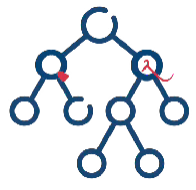
\includegraphics[height=0.9cm]{msca_logo.png}}%
  \end{center}
  \vspace{0.45cm}
  \begin{center}
    \begin{minipage}{0.1\textwidth}\centering
      \href{https://quantlet.com}{
\includegraphics[height=0.9cm]{ql_logo.png}}\end{minipage}%
    \begin{minipage}{0.78\textwidth}\centering
      {\Large\bfseries\usebeamercolor[fg]{title}\inserttitle}\par\vspace{0.25cm}
      {\large\usebeamercolor[fg]{title}\insertsubtitle}\end{minipage}%
    \begin{minipage}{0.1\textwidth}\centering
      \href{https://quantinar.com}{
\includegraphics[height=0.9cm]{qr_logo.png}}\end{minipage}
  \end{center}
  \vfill
  \hspace{0.4cm}{\bfseries\insertauthor}\par\vspace{0.12cm}
  \hspace{0.4cm}\begin{minipage}[t]{0.92\textwidth}\raggedright\footnotesize\insertinstitute\end{minipage}
  \par\vspace{0.4cm}}

% ---------------------------------------------------------------- lecture metadata
\newcommand{\nnshort}{}
\newcommand{\nnnb}{notebooks}
\newcommand{\nnrepo}{https://github.com/danpele/NEURAL_BIZ/tree/main}
% language-dependent labels (English default; \nnromanian switches to Romanian, call it before \nnlecture)
\newcommand{\txtcourse}{Neural Networks and Deep Learning}
\newcommand{\txtlecture}{Lecture}
\newcommand{\txtoutline}{Outline}
\newcommand{\txtintuition}{In one sentence:}
\newcommand{\txtjob}{In practice:}
\newcommand{\txttry}{Experiment yourself:}
\newcommand{\txtwhere}{where}
\newcommand{\txtsim}{SIMULATED DATA (teaching illustration)}
\newcommand{\txtnbsuffix}{}
\newcommand{\txtinstitute}{Bucharest University of Economic Studies (ASE), Department of Statistics and Econometrics\\
    Romanian Academy, Institute for Economic Forecasting (IPE)\\
    IDA Institute Digital Assets \textbullet\ AI4EFin \textbullet\ MSCA Digital Finance}
\newcommand{\nnromanian}{%
  \renewcommand{\txtcourse}{Rețele neuronale și deep learning}%
  \renewcommand{\txtlecture}{Cursul}%
  \renewcommand{\txtoutline}{Cuprins}%
  \renewcommand{\txtintuition}{Pe scurt:}%
  \renewcommand{\txtjob}{În practică:}%
  \renewcommand{\txttry}{Exercițiu practic:}%
  \renewcommand{\txtwhere}{unde}%
  \renewcommand{\txtsim}{DATE SIMULATE (doar pentru ilustrare)}%
  \renewcommand{\txtnbsuffix}{\string_ro}%
  \renewcommand{\txtinstitute}{Academia de Studii Economice din București (ASE), Departamentul de Statistică și Econometrie\\
    Academia Română, Institutul de Prognoză Economică (IPE)\\
    IDA Institute Digital Assets \textbullet\ AI4EFin \textbullet\ MSCA Digital Finance}}
\newcommand{\nnlecture}[2]{%
  \renewcommand{\nnshort}{\txtlecture\ #1}%
  \renewcommand{\nnnb}{notebooks/L#1\string_notebook\txtnbsuffix.ipynb}%
  \title[NN]{\txtcourse}%
  \subtitle{\txtlecture\ #1: #2}%
  \author{Prof.\ dr.\ Daniel Traian PELE}%
  \institute{\txtinstitute}%
  \date{}}

% ---------------------------------------------------------------- teaching blocks (one message per frame)
% \intuition{one plain sentence}  ->  formula with every symbol defined  ->  real-data example  ->  \manager{one line}
\newcommand{\intuition}[1]{\begin{itemize}\item {\color{MainBlue}\textbf{\txtintuition}}~#1\end{itemize}\vspace{0.6mm}}
\newcommand{\manager}[1]{\colorbox{Forest!10}{\parbox{\dimexpr\linewidth-2\fboxsep\relax}{\footnotesize
  \begin{itemize}\setlength{\itemsep}{0pt}\item \textbf{\color{Forest}\txtjob}~#1\end{itemize}}}}
% Experiment yourself: pointer to the matching notebook section
\newcommand{\tryit}[1]{{\scriptsize\href{\nnrepo/\nnnb}{%
  \raisebox{-0.15em}{
\includegraphics[height=0.85em]{ql_logo.png}}\,\textbf{\txttry}~\color{MainBlue}#1}}}
% bottom row: manager line (left) + experiment pointer (right), pinned to the bottom of the frame
\newcommand{\bottomrow}[2]{\par\vfill\noindent\begin{minipage}[b]{0.72\linewidth}#1\end{minipage}\hfill
  \begin{minipage}[b]{0.26\linewidth}\raggedleft #2\end{minipage}\par\vspace{0.5mm}}
\newcommand{\where}[1]{{\footnotesize\textbf{\txtwhere}~#1\par}}

% ---------------------------------------------------------------- helpers
% chart source line under a figure: \chartsource{Source ...; period ...}
\newcommand{\chartsource}[1]{\par\vspace{1pt}{\scriptsize\color{FooterGray}#1\par}}
% link to code: \quantlet{label}{path inside the repo}
\newcommand{\quantlet}[2]{\par\vspace{1pt}\hfill\href{\nnrepo/#2}{%
  \raisebox{-0.15em}{
\includegraphics[height=0.75em]{ql_logo.png}}\textcolor{MainBlue}{\scriptsize\ #1}}}
% inline Quantlet link for the bottom-right corner of a frame: \qlink{label}{path inside the repo}
\newcommand{\qlink}[2]{{\scriptsize\href{\nnrepo/#2}{\raisebox{-0.15em}{
\includegraphics[height=0.85em]{ql_logo.png}}\,\textcolor{MainBlue}{#1}}}}
\newcommand{\simlabel}{\colorbox{Crimson!12}{\scriptsize\bfseries\color{Crimson}\txtsim}}
\newcommand{\E}{\mathbb{E}}
\newcommand{\Var}{\operatorname{Var}}
\newcommand{\Cov}{\operatorname{Cov}}
\newcommand{\Corr}{\operatorname{Corr}}
\newcommand{\asinh}{\operatorname{asinh}}
\newcommand{\iid}{\overset{\text{i.i.d.}}{\sim}}
\newcommand{\EUR}{EUR}
% deep-learning notation (Bishop & Bishop, 2024): vectors bold lower case, matrices bold upper case
\newcommand{\R}{\mathbb{R}}
\newcommand{\vx}{\mathbf{x}}
\newcommand{\vy}{\mathbf{y}}
\newcommand{\vz}{\mathbf{z}}
\newcommand{\vh}{\mathbf{h}}
\newcommand{\vw}{\mathbf{w}}
\newcommand{\vb}{\mathbf{b}}
\newcommand{\mW}{\mathbf{W}}
\newcommand{\mX}{\mathbf{X}}
\newcommand{\btheta}{\boldsymbol{\theta}}
\newcommand{\loss}{\mathcal{L}}
\newcommand{\dataset}{\mathcal{D}}
\DeclareMathOperator*{\argmin}{arg\,min}
\DeclareMathOperator*{\argmax}{arg\,max}
\DeclareMathOperator{\softmax}{softmax}
\DeclareMathOperator{\ReLU}{ReLU}
\DeclareMathOperator{\sigm}{\sigma}

%   \nnlecture{k}{Lecture title}
% Logos live in lectures/common/logos/, charts in lectures/Lk/charts/.
% Do NOT add \hfuzz / \vfuzz / \hbadness here: overfull boxes must be fixed, not hidden.
% =============================================================================

\usetheme{default}
\setbeamersize{text margin left=7mm, text margin right=7mm}

% ---------------------------------------------------------------- packages
\usepackage[utf8]{inputenc}
\usepackage[T1]{fontenc}
\usepackage{lmodern}
\usepackage{amsmath, amssymb}
\usepackage{mathtools}
\usepackage{bm}
\usepackage{tikz}
\usetikzlibrary{arrows.meta, positioning, calc, shapes.misc}
\usepackage{booktabs}
\usepackage{array}
\usepackage{graphicx}
\usepackage{colortbl}
\usepackage{xcolor}
\usepackage{multicol}
\hypersetup{colorlinks=true, linkcolor=MainBlue, urlcolor=MainBlue, citecolor=MainBlue}
\graphicspath{{../common/logos/}}   % charts are included with their language folder: charts/en/, charts/ro/

% ---------------------------------------------------------------- colours
\definecolor{MainBlue}{RGB}{26, 58, 110}
\definecolor{IDAred}{RGB}{205, 0, 0}
\definecolor{DarkGray}{RGB}{51, 51, 51}
\definecolor{FooterGray}{RGB}{100, 100, 100}
\definecolor{BlockGray}{RGB}{236, 238, 242}
\definecolor{KeynoteGray}{RGB}{218, 218, 218}
\definecolor{Crimson}{RGB}{190, 40, 50}
\definecolor{Forest}{RGB}{30, 110, 50}
\definecolor{Bitter}{RGB}{214, 150, 20}
% chart palette (same hex values and order as lectures/common/nn_plot.py SERIES)
\definecolor{Ser1}{HTML}{2A78D6}
\definecolor{Ser2}{HTML}{EB6834}
\definecolor{Ser3}{HTML}{1BAF7A}
\definecolor{Ser4}{HTML}{EDA100}
\definecolor{Ser5}{HTML}{E87BA4}
\definecolor{Ser6}{HTML}{008300}
\definecolor{Ser7}{HTML}{6250D6}
\definecolor{Ser8}{HTML}{E34948}

\setbeamertemplate{background}{%
  \begin{tikzpicture}[remember picture, overlay]
    \shade[shading=axis, shading angle=315, top color=white, bottom color=KeynoteGray]
      (current page.south west) rectangle (current page.north east);
  \end{tikzpicture}}
\setbeamercolor{background canvas}{bg=}
\setbeamercolor{structure}{fg=MainBlue}
\setbeamercolor{normal text}{fg=DarkGray}
\setbeamercolor{title}{fg=IDAred}
\setbeamercolor{frametitle}{fg=IDAred, bg=}
\setbeamercolor{block title}{bg=MainBlue, fg=white}
\setbeamercolor{block body}{bg=BlockGray, fg=DarkGray}
\setbeamercolor{block title alerted}{bg=Crimson, fg=white}
\setbeamercolor{block body alerted}{bg=Crimson!7, fg=DarkGray}
\setbeamercolor{block title example}{bg=Forest, fg=white}
\setbeamercolor{block body example}{bg=Forest!7, fg=DarkGray}
\setbeamercolor{item}{fg=MainBlue}
\setbeamerfont{frametitle}{size=\large, series=\bfseries}
\setbeamerfont{block title}{size=\small, series=\bfseries}
\setbeamertemplate{blocks}[rounded][shadow=false]
\setbeamertemplate{itemize item}{\color{MainBlue}$\boxdot$}
\setbeamertemplate{itemize subitem}{\color{MainBlue}\scriptsize$\blacktriangleright$}
% compact two-level lists: level 1 = main point, level 2 = details (no text outside bullets)
\setbeamerfont{itemize/enumerate subbody}{size=\footnotesize}
\setlength{\leftmargini}{1.1em}
\setlength{\leftmarginii}{1.1em}
\setbeamertemplate{itemize/enumerate body begin}{\setlength{\topsep}{0pt}\setlength{\partopsep}{0pt}\setlength{\parskip}{0pt}}
\setbeamertemplate{itemize/enumerate subbody begin}{\setlength{\topsep}{0pt}\setlength{\partopsep}{0pt}\setlength{\itemsep}{0pt}\vspace{-0.4ex}}

\setbeamertemplate{enumerate item}{\color{MainBlue}\insertenumlabel.}
\setlength{\leftmargini}{1.3em}
\setlength{\leftmarginii}{1.2em}
\setbeamertemplate{navigation symbols}{}
\setbeamertemplate{section in toc}{\color{MainBlue}$\blacktriangleright$~\inserttocsection}
\setbeamertemplate{caption}{\raggedright\insertcaption\par}
% frame subtitle = precise citation line under the claim title (Weron style)
\setbeamerfont{framesubtitle}{size=\footnotesize}
\setbeamercolor{framesubtitle}{fg=FooterGray}
% outline that reappears at every section with the current section highlighted
\setbeamertemplate{section in toc shaded}[default][35]
\setbeamertemplate{subsection in toc shaded}[default][35]
\setbeamertemplate{subsection in toc}{\leavevmode\leftskip=2.2em\color{DarkGray}\small\inserttocsubsection\par}
\AtBeginSection[]{{\begin{frame}{\txtoutline}\vspace{2mm}\small
  \tableofcontents[currentsection,hideothersubsections]\end{frame}}}

% ---------------------------------------------------------------- head and foot
\setbeamertemplate{headline}{%
  \vskip10pt%
  \hbox to \paperwidth{\hskip0.5cm%
    {\small\color{FooterGray}\renewcommand{\hyperlink}[2]{##2}\insertsectionhead}%
    \hfill\textcolor{FooterGray}{\small\insertframenumber}\hskip0.5cm}%
  \vskip4pt{\color{FooterGray}\hrule height 0.4pt}}
% footer as in the other courses (MFM, SFM): course name on the left, small sparkline on the right
\setbeamertemplate{footline}{%
  {\color{FooterGray}\hrule height 0.4pt}\vskip4pt%
  \hbox to \paperwidth{\hskip0.5cm%
    \textcolor{FooterGray}{\small\txtcourse}%
    \hfill\raisebox{-0.1em}{\begin{tikzpicture}[x=0.08em, y=0.08em, line width=0.4pt]
      \draw[FooterGray] (0,3) -- (1,4) -- (2,3.5) -- (3,5) -- (4,4) -- (5,6) -- (6,5.5) -- (7,4) -- (8,5) -- (9,7) -- (10,6) -- (11,5) -- (12,6.5) -- (13,8) -- (14,7) -- (15,6) -- (16,7.5) -- (17,9) -- (18,8) -- (19,7) -- (20,8.5) -- (21,10) -- (22,9) -- (23,8) -- (24,9.5);
    \end{tikzpicture}}\hskip0.5cm}%
  \vskip6pt}

% ---------------------------------------------------------------- title page
\defbeamertemplate*{title page}{nn}[1][]{%
  \vspace{0.15cm}
  \begin{center}
    \href{https://www.ase.ro}{
\includegraphics[height=0.9cm]{ase_logo.png}}\hspace{0.3cm}%
    \href{https://ipe.ro/new}{
\includegraphics[height=0.9cm]{acad_logo.png}}\hspace{0.3cm}%
    \href{https://theida.net}{
\includegraphics[height=0.9cm]{ida_logo.png}}\hspace{0.3cm}%
    \href{https://blockchain-research-center.com}{
\includegraphics[height=0.9cm]{brc_logo.png}}\hspace{0.3cm}%
    \href{https://www.ai4efin.ase.ro}{
\includegraphics[height=0.9cm]{ai4efin_logo.png}}\hspace{0.3cm}%
    \href{https://www.digital-finance-msca.com}{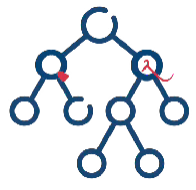
\includegraphics[height=0.9cm]{msca_logo.png}}%
  \end{center}
  \vspace{0.45cm}
  \begin{center}
    \begin{minipage}{0.1\textwidth}\centering
      \href{https://quantlet.com}{
\includegraphics[height=0.9cm]{ql_logo.png}}\end{minipage}%
    \begin{minipage}{0.78\textwidth}\centering
      {\Large\bfseries\usebeamercolor[fg]{title}\inserttitle}\par\vspace{0.25cm}
      {\large\usebeamercolor[fg]{title}\insertsubtitle}\end{minipage}%
    \begin{minipage}{0.1\textwidth}\centering
      \href{https://quantinar.com}{
\includegraphics[height=0.9cm]{qr_logo.png}}\end{minipage}
  \end{center}
  \vfill
  \hspace{0.4cm}{\bfseries\insertauthor}\par\vspace{0.12cm}
  \hspace{0.4cm}\begin{minipage}[t]{0.92\textwidth}\raggedright\footnotesize\insertinstitute\end{minipage}
  \par\vspace{0.4cm}}

% ---------------------------------------------------------------- lecture metadata
\newcommand{\nnshort}{}
\newcommand{\nnnb}{notebooks}
\newcommand{\nnrepo}{https://github.com/danpele/NEURAL_BIZ/tree/main}
% language-dependent labels (English default; \nnromanian switches to Romanian, call it before \nnlecture)
\newcommand{\txtcourse}{Neural Networks and Deep Learning}
\newcommand{\txtlecture}{Lecture}
\newcommand{\txtoutline}{Outline}
\newcommand{\txtintuition}{In one sentence:}
\newcommand{\txtjob}{In practice:}
\newcommand{\txttry}{Experiment yourself:}
\newcommand{\txtwhere}{where}
\newcommand{\txtsim}{SIMULATED DATA (teaching illustration)}
\newcommand{\txtnbsuffix}{}
\newcommand{\txtinstitute}{Bucharest University of Economic Studies (ASE), Department of Statistics and Econometrics\\
    Romanian Academy, Institute for Economic Forecasting (IPE)\\
    IDA Institute Digital Assets \textbullet\ AI4EFin \textbullet\ MSCA Digital Finance}
\newcommand{\nnromanian}{%
  \renewcommand{\txtcourse}{Rețele neuronale și deep learning}%
  \renewcommand{\txtlecture}{Cursul}%
  \renewcommand{\txtoutline}{Cuprins}%
  \renewcommand{\txtintuition}{Pe scurt:}%
  \renewcommand{\txtjob}{În practică:}%
  \renewcommand{\txttry}{Exercițiu practic:}%
  \renewcommand{\txtwhere}{unde}%
  \renewcommand{\txtsim}{DATE SIMULATE (doar pentru ilustrare)}%
  \renewcommand{\txtnbsuffix}{\string_ro}%
  \renewcommand{\txtinstitute}{Academia de Studii Economice din București (ASE), Departamentul de Statistică și Econometrie\\
    Academia Română, Institutul de Prognoză Economică (IPE)\\
    IDA Institute Digital Assets \textbullet\ AI4EFin \textbullet\ MSCA Digital Finance}}
\newcommand{\nnlecture}[2]{%
  \renewcommand{\nnshort}{\txtlecture\ #1}%
  \renewcommand{\nnnb}{notebooks/L#1\string_notebook\txtnbsuffix.ipynb}%
  \title[NN]{\txtcourse}%
  \subtitle{\txtlecture\ #1: #2}%
  \author{Prof.\ dr.\ Daniel Traian PELE}%
  \institute{\txtinstitute}%
  \date{}}

% ---------------------------------------------------------------- teaching blocks (one message per frame)
% \intuition{one plain sentence}  ->  formula with every symbol defined  ->  real-data example  ->  \manager{one line}
\newcommand{\intuition}[1]{\begin{itemize}\item {\color{MainBlue}\textbf{\txtintuition}}~#1\end{itemize}\vspace{0.6mm}}
\newcommand{\manager}[1]{\colorbox{Forest!10}{\parbox{\dimexpr\linewidth-2\fboxsep\relax}{\footnotesize
  \begin{itemize}\setlength{\itemsep}{0pt}\item \textbf{\color{Forest}\txtjob}~#1\end{itemize}}}}
% Experiment yourself: pointer to the matching notebook section
\newcommand{\tryit}[1]{{\scriptsize\href{\nnrepo/\nnnb}{%
  \raisebox{-0.15em}{
\includegraphics[height=0.85em]{ql_logo.png}}\,\textbf{\txttry}~\color{MainBlue}#1}}}
% bottom row: manager line (left) + experiment pointer (right), pinned to the bottom of the frame
\newcommand{\bottomrow}[2]{\par\vfill\noindent\begin{minipage}[b]{0.72\linewidth}#1\end{minipage}\hfill
  \begin{minipage}[b]{0.26\linewidth}\raggedleft #2\end{minipage}\par\vspace{0.5mm}}
\newcommand{\where}[1]{{\footnotesize\textbf{\txtwhere}~#1\par}}

% ---------------------------------------------------------------- helpers
% chart source line under a figure: \chartsource{Source ...; period ...}
\newcommand{\chartsource}[1]{\par\vspace{1pt}{\scriptsize\color{FooterGray}#1\par}}
% link to code: \quantlet{label}{path inside the repo}
\newcommand{\quantlet}[2]{\par\vspace{1pt}\hfill\href{\nnrepo/#2}{%
  \raisebox{-0.15em}{
\includegraphics[height=0.75em]{ql_logo.png}}\textcolor{MainBlue}{\scriptsize\ #1}}}
% inline Quantlet link for the bottom-right corner of a frame: \qlink{label}{path inside the repo}
\newcommand{\qlink}[2]{{\scriptsize\href{\nnrepo/#2}{\raisebox{-0.15em}{
\includegraphics[height=0.85em]{ql_logo.png}}\,\textcolor{MainBlue}{#1}}}}
\newcommand{\simlabel}{\colorbox{Crimson!12}{\scriptsize\bfseries\color{Crimson}\txtsim}}
\newcommand{\E}{\mathbb{E}}
\newcommand{\Var}{\operatorname{Var}}
\newcommand{\Cov}{\operatorname{Cov}}
\newcommand{\Corr}{\operatorname{Corr}}
\newcommand{\asinh}{\operatorname{asinh}}
\newcommand{\iid}{\overset{\text{i.i.d.}}{\sim}}
\newcommand{\EUR}{EUR}
% deep-learning notation (Bishop & Bishop, 2024): vectors bold lower case, matrices bold upper case
\newcommand{\R}{\mathbb{R}}
\newcommand{\vx}{\mathbf{x}}
\newcommand{\vy}{\mathbf{y}}
\newcommand{\vz}{\mathbf{z}}
\newcommand{\vh}{\mathbf{h}}
\newcommand{\vw}{\mathbf{w}}
\newcommand{\vb}{\mathbf{b}}
\newcommand{\mW}{\mathbf{W}}
\newcommand{\mX}{\mathbf{X}}
\newcommand{\btheta}{\boldsymbol{\theta}}
\newcommand{\loss}{\mathcal{L}}
\newcommand{\dataset}{\mathcal{D}}
\DeclareMathOperator*{\argmin}{arg\,min}
\DeclareMathOperator*{\argmax}{arg\,max}
\DeclareMathOperator{\softmax}{softmax}
\DeclareMathOperator{\ReLU}{ReLU}
\DeclareMathOperator{\sigm}{\sigma}

\usepackage[romanian]{babel}
\nnromanian
\nnlecture{9}{Rețele neuronale pe grafuri}
\begin{document}
{\setbeamertemplate{headline}{}\setbeamertemplate{footline}{}
\begin{frame}\titlepage\end{frame}}
% END-FRONT-MATTER

\begin{frame}{Obiectivele cursului}
\small
\begin{itemize}\setlength{\itemsep}{5pt}
  \item Reprezentarea datelor financiare ca graf
    \begin{itemize}\setlength{\itemsep}{0pt}
      \item Noduri, muchii și variabilele nodurilor
      \item Matricea de adiacență, matricea gradelor și adiacența normalizată
    \end{itemize}
  \item Schema de transmitere a mesajelor a unei rețele neuronale pe graf (GNN)
    \begin{itemize}\setlength{\itemsep}{0pt}
      \item Cele trei straturi clasice: rețeaua convoluțională pe graf (GCN), eșantionarea și agregarea pe graf (GraphSAGE), rețeaua cu atenție pe graf (GAT)
    \end{itemize}
  \item Antrenarea lor pe graful Bitcoin Elliptic pentru combaterea spălării banilor (AML), în ordine cronologică
    \begin{itemize}\setlength{\itemsep}{0pt}
      \item Comparația cu regresia logistică și cu pădurea aleatoare
    \end{itemize}
  \item Evaluarea rezultatelor ca un investigator
    \begin{itemize}\setlength{\itemsep}{0pt}
      \item Precizia, recall-ul și aria de sub curba precizie-recall (PR-AUC)
      \item Alertele pe analist, schimbarea în timp și stabilitatea explicațiilor
    \end{itemize}
\end{itemize}
\end{frame}

% BEGIN-ABBR

\begin{frame}{Abrevieri}
\small
\vspace{-1mm}\begin{columns}[T,onlytextwidth]
\begin{column}{0.49\textwidth}{\scriptsize\renewcommand{\arraystretch}{0.96}\begin{tabular}{@{}>{\bfseries}l@{\ \ }p{0.74\linewidth}@{}}AML & combaterea spălării banilor (anti-money laundering)\\
ASE & Academia de Studii Economice din București\\
BTC & bitcoin (unitate monetară)\\
CNN & rețea neuronală convoluțională\\
CPU & unitate centrală de procesare\\
GAT & rețea cu atenție pe graf (graph attention network)\\
GCN & rețea convoluțională pe graf (graph convolutional network)\\
GIN & rețea de izomorfism pe graf (graph isomorphism network)\\
GNN & rețea neuronală pe graf (graph neural network)\\
GraphSAGE & eșantionare și agregare pe graf (graph sample and aggregate)\\\end{tabular}}\end{column}
\begin{column}{0.49\textwidth}{\scriptsize\renewcommand{\arraystretch}{0.96}\begin{tabular}{@{}>{\bfseries}l@{\ \ }p{0.74\linewidth}@{}}IPE & Institutul de Prognoză Economică, Academia Română\\
MLP & perceptron multistrat\\
MPNN & rețea neuronală cu transmitere de mesaje (message passing)\\
PCA & analiza componentelor principale\\
PR-AUC & aria de sub curba precizie-recall\\
PyG & PyTorch Geometric (bibliotecă de programe)\\
ReLU & unitate liniară rectificată (rectified linear unit)\\
SHAP & explicații aditive bazate pe valorile Shapley (SHapley Additive exPlanations)\\
WL & testul de izomorfism Weisfeiler--Leman\\
XAI & inteligență artificială explicabilă\\\end{tabular}}\end{column}
\end{columns}
\end{frame}

% END-ABBR


\section{De ce grafuri pentru infracțiunile financiare}

\begin{frame}{Spălarea banilor se ascunde în legături, nu în rînduri}
\footnotesize
\intuition{O plată izolată poate părea obișnuită; lanțul de plăți din jurul ei, de cele mai multe ori, nu.}
\begin{columns}[T,onlytextwidth]
\begin{column}{0.53\textwidth}
\[ G=(\mathcal V,\mathcal E,\mathbf X),\qquad \mathbf X\in\R^{n\times d},\qquad y_v\in\{0,1\} \]{\footnotesize\begin{itemize}\setlength{\itemsep}{0pt}
  \item \textbf{\txtwhere}
    \begin{itemize}\setlength{\itemsep}{0pt}
      \item $\mathcal V$ = nodurile (tranzacțiile), $n=|\mathcal V|$
      \item $\mathcal E$ = muchiile (un flux de plată de la o tranzacție la următoarea)
      \item $\mathbf X$ = variabilele nodurilor, cîte $d$ pentru fiecare nod
      \item $y_v=1$ dacă tranzacția $v$ este ilicită.
    \end{itemize}
\end{itemize}\par}
\end{column}
\begin{column}{0.44\textwidth}
\begin{itemize}\setlength{\itemsep}{3pt}
  \item \textbf{Graful Elliptic} (Weber et al., 2019)
    \begin{itemize}\setlength{\itemsep}{0pt}
      \item 203\,769 de tranzacții Bitcoin, 234\,355 de fluxuri de plată
      \item 165 de variabile pe tranzacție, 49 de pași de timp
    \end{itemize}
  \item \textbf{Sarcina}
    \begin{itemize}\setlength{\itemsep}{0pt}
      \item Clasificarea nodurilor: ilicit (fraude, ransomware, piețe ilegale) sau licit
    \end{itemize}
\end{itemize}
\end{column}
\end{columns}
\par\vfill\manager{echipa de conformitate a unei bănci gîndește deja în lanțuri de plăți
    \begin{itemize}\setlength{\itemsep}{0pt}
      \item O rețea GNN învață din aceleași lanțuri.
    \end{itemize}}\par\vspace{0.5mm}
\par\vfill\noindent{\scriptsize\color{FooterGray}(Weber et al., 2019; Bishop \& Bishop, 2024, ch.\ 13)}\hfill\tryit{notebook, secțiunea 1}\par\vspace{0.5mm}
\end{frame}

\begin{frame}{Datele Elliptic într-un singur tabel}
\footnotesize
{\scriptsize\renewcommand{\arraystretch}{1.05}\setlength{\tabcolsep}{4pt}
\begin{tabular}{@{}p{0.30\textwidth}p{0.62\textwidth}@{}}\toprule
Element & Valoarea în copia noastră a datelor \\ \midrule
Noduri, muchii & 203\,769 de tranzacții; 234\,355 de fluxuri de plată orientate \\
Etichete & 4\,545 ilicite, 42\,019 licite, 157\,205 necunoscute (22{,}9\,\% etichetate) \\
Variabile & 93 locale (sume, comisioane, intrări, ieșiri) și 72 agregate pe vecini \\
Timpul & 49 de pași de circa două săptămîni; muchiile leagă tranzacții din același pas (100{,}0\,\%) \\
Antrenare / test & pașii 1--34 (29\,894 etichetate) / pașii 35--49 (16\,670 etichetate, 1\,083 ilicite) \\
\bottomrule\end{tabular}}
\vspace{1mm}
\begin{itemize}\setlength{\itemsep}{2pt}
  \item \textbf{Dezechilibrul claselor}: doar 9{,}76\,\% dintre tranzacțiile etichetate sînt ilicite
    \begin{itemize}\setlength{\itemsep}{0pt}
      \item Acuratețea singură nu spune nimic
    \end{itemize}
  \item \textbf{Date anonimizate}: Elliptic nu publică denumirile variabilelor
    \begin{itemize}\setlength{\itemsep}{0pt}
      \item Le notăm $f_1,\dots,f_{165}$
    \end{itemize}
\end{itemize}
\par\vfill\noindent{\scriptsize\color{FooterGray}(Weber et al., 2019)}\hfill\tryit{notebook, secțiunea 1}\par\vspace{0.5mm}
\end{frame}

\begin{frame}{Etichetele vin în valuri: activitatea ilicită nu este staționară}
\small
\begin{center}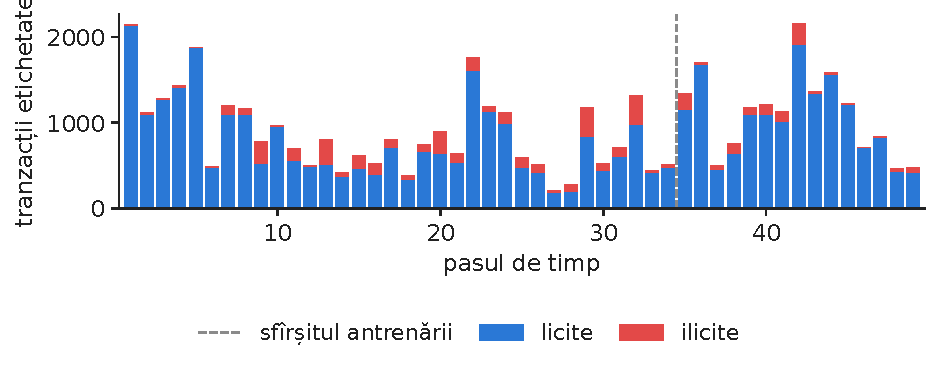
\includegraphics[width=\textwidth,height=0.389\textheight,keepaspectratio]{charts/ro/elliptic_timesteps.pdf}\end{center}\vspace{-3mm}
\chartsource{Sursa: Graful tranzacțiilor Bitcoin Elliptic (Weber et al., 2019). Date: graful tranzacțiilor Bitcoin Elliptic, 49 de pași de timp (circa două săptămîni fiecare).}
\vspace{0.5mm}
\begin{itemize}\setlength{\itemsep}{0pt}
  \item \textbf{Vîrful}: 342 de tranzacții ilicite în pasul 32
    \begin{itemize}\setlength{\itemsep}{0pt}
      \item În medie, circa 4\,159 de tranzacții pe pas
    \end{itemize}
  \item \textbf{Împărțire în timp}: antrenare pe pașii 1--34, test o singură dată pe pașii 35--49, ca în Weber et al.\ (2019)
    \begin{itemize}\setlength{\itemsep}{0pt}
      \item Pașii nu se amestecă
    \end{itemize}
\end{itemize}
\par\vfill\manager{un model este judecat pe lunile de după datele de antrenare, exact cum va fi folosit.}\par\vspace{0.5mm}
\par\vfill\noindent{\scriptsize\color{FooterGray}}\hfill\qlink{NN\_L9\_elliptic\_timesteps}{Quantlets/L9/NN_L9_elliptic_timesteps}\par\vspace{0.5mm}
\end{frame}

\begin{frame}{Cele mai multe tranzacții ating una sau două altele; puține sînt noduri centrale}
\small
\begin{center}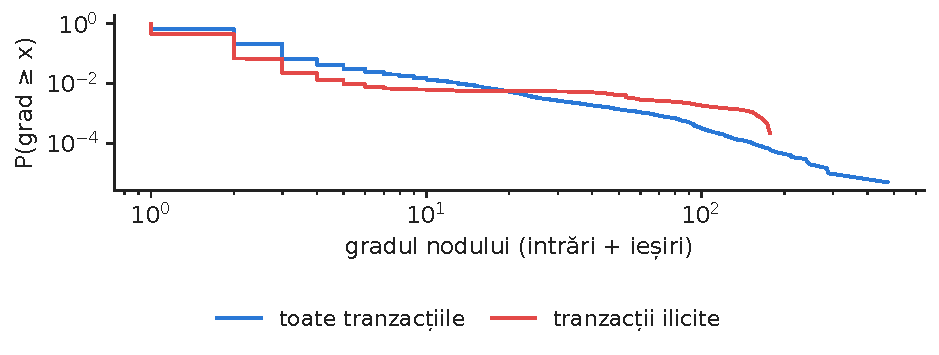
\includegraphics[width=\textwidth,height=0.519\textheight,keepaspectratio]{charts/ro/degree_dist.pdf}\end{center}\vspace{-3mm}
\chartsource{Sursa: Graful tranzacțiilor Bitcoin Elliptic (Weber et al., 2019). Date: graful tranzacțiilor Bitcoin Elliptic, 49 de pași de timp (circa două săptămîni fiecare).}
\vspace{0.5mm}
\begin{itemize}\setlength{\itemsep}{0pt}
  \item \textbf{Graf rar}: gradul mediu 2{,}30, mediana 2
    \begin{itemize}\setlength{\itemsep}{0pt}
      \item 34{,}5\,\% dintre noduri au un singur vecin
    \end{itemize}
  \item \textbf{Coadă grea}: cel mai mare nod central are 473 de vecini
    \begin{itemize}\setlength{\itemsep}{0pt}
      \item O rețea GNN nu trebuie să lase nodurile centrale să le acopere pe celelalte (de aici normalizarea)
    \end{itemize}
\end{itemize}
\par\vfill\noindent{\scriptsize\color{FooterGray}$\deg(v)=|\mathcal N(v)|$}\hfill\qlink{NN\_L9\_degree\_dist}{Quantlets/L9/NN_L9_degree_dist}\par\vspace{0.5mm}
\end{frame}

\begin{frame}{Tranzacțiile ilicite stau lîngă alte tranzacții ilicite}
\small
\begin{center}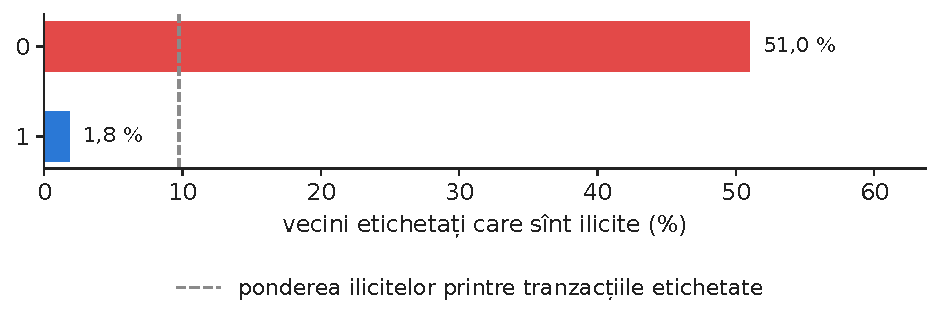
\includegraphics[width=\textwidth,height=0.480\textheight,keepaspectratio]{charts/ro/homophily.pdf}\end{center}\vspace{-3mm}
\chartsource{Sursa: Graful tranzacțiilor Bitcoin Elliptic (Weber et al., 2019). Date: graful tranzacțiilor Bitcoin Elliptic, 49 de pași de timp (circa două săptămîni fiecare).}
\vspace{0.5mm}
\begin{itemize}\setlength{\itemsep}{0pt}
  \item \textbf{Homofilie}: 51{,}0\,\% dintre vecinii etichetați ai unui nod ilicit sînt ilicite, față de 1{,}8\,\% pentru un nod licit
  \item \textbf{Homofilia muchiilor}: 95{,}4\,\% dintre muchiile etichetate leagă noduri din aceeași clasă
    \begin{itemize}\setlength{\itemsep}{0pt}
      \item Cu etichete aleatoare: 82{,}4\,\%
    \end{itemize}
\end{itemize}
\par\vfill\manager{homofilia este motivul pentru care ne uităm la vecini: cu cine tranzacționezi spune ceva despre tine.}\par\vspace{0.5mm}
\par\vfill\noindent{\scriptsize\color{FooterGray}}\hfill\qlink{NN\_L9\_homophily}{Quantlets/L9/NN_L9_homophily}\par\vspace{0.5mm}
\end{frame}


\section{Grafurile ca matrice}

\begin{frame}{Matricea de adiacență transformă graful în algebră liniară}
\footnotesize
\intuition{Orice operație a unei rețele GNN este un produs între matricea variabilelor, o matrice de adiacență (normalizată) și o matrice de ponderi.}
\begin{columns}[T,onlytextwidth]
\begin{column}{0.53\textwidth}
\[ A_{uv}=\begin{cases}1,&(u,v)\in\mathcal E\\0,&\text{altfel}\end{cases},\qquad D=\operatorname{diag}\Big(\sum_v A_{uv}\Big) \]\[ \tilde A=A+I,\qquad \hat A=\tilde D^{-1/2}\tilde A\,\tilde D^{-1/2} \]{\footnotesize\begin{itemize}\setlength{\itemsep}{0pt}
  \item \textbf{\txtwhere}
    \begin{itemize}\setlength{\itemsep}{0pt}
      \item $A$ = matricea de adiacență, simetrizată
      \item $D$ = matricea gradelor
      \item $\tilde A$ adaugă bucle (nodul își păstrează variabilele)
      \item $\hat A$ are elementele $1/\sqrt{\tilde d_u\tilde d_v}$.
    \end{itemize}
\end{itemize}\par}
\end{column}
\begin{column}{0.44\textwidth}
\begin{itemize}\setlength{\itemsep}{3pt}
  \item \textbf{Stocare rară}
    \begin{itemize}\setlength{\itemsep}{0pt}
      \item $A$ are $n^2\approx 4\cdot 10^{10}$ celule, dar numai 234\,355 de muchii
      \item Bibliotecile păstrează o listă de muchii $2\times|\mathcal E|$, ca PyTorch Geometric (PyG)
    \end{itemize}
  \item \textbf{De ce normalizăm}
    \begin{itemize}\setlength{\itemsep}{0pt}
      \item Fără normalizare, un nod central de grad 473 ar aduna 473 de mesaje, iar scala ar exploda
    \end{itemize}
\end{itemize}
\end{column}
\end{columns}
\par\vfill\manager{rețeaua de plăți a unei bănci se stochează ca listă de muchii, niciodată ca matrice densă.}\par\vspace{0.5mm}
\par\vfill\noindent{\scriptsize\color{FooterGray}(Kipf \& Welling, 2017)}\hfill\tryit{notebook, secțiunea 2}\par\vspace{0.5mm}
\end{frame}

\begin{frame}{Un model pe graf nu trebuie să depindă de numerotarea nodurilor}
\footnotesize
\intuition{Tranzacția 17 și tranzacția 4.203 sînt nume, nu poziții; renumerotarea lor nu trebuie să schimbe nicio predicție.}
\begin{columns}[T,onlytextwidth]
\begin{column}{0.53\textwidth}
\[ f\big(P\mathbf X,\;PAP^{\top}\big)=P\,f(\mathbf X,A)\quad\forall P \]{\footnotesize\begin{itemize}\setlength{\itemsep}{0pt}
  \item \textbf{\txtwhere}
    \begin{itemize}\setlength{\itemsep}{0pt}
      \item $P$ = orice matrice de permutare $n\times n$
      \item $f$ dă cîte un rînd de rezultate pentru fiecare nod: \textit{echivarianță}
      \item Un rezultat la nivelul întregului graf trebuie să fie \textit{invariant}: $g(P\mathbf X,PAP^{\top})=g(\mathbf X,A)$.
    \end{itemize}
\end{itemize}\par}
\end{column}
\begin{column}{0.44\textwidth}
\begin{itemize}\setlength{\itemsep}{3pt}
  \item \textbf{De ce nu un perceptron multistrat (MLP)?}
    \begin{itemize}\setlength{\itemsep}{0pt}
      \item Pe rîndurile lui $A$ ar avea nevoie de $n$ intrări și s-ar schimba odată cu numerotarea
    \end{itemize}
  \item \textbf{De ce nu o rețea neuronală convoluțională (CNN)?}
    \begin{itemize}\setlength{\itemsep}{0pt}
      \item Presupune o grilă cu un număr fix de vecini ordonați
      \item Un nod are între 1 și 473 de vecini, fără nicio ordine
    \end{itemize}
\end{itemize}
\end{column}
\end{columns}
\par\vfill\manager{întrebați despre orice model cumpărat: se schimbă scorul dacă fișierul de intrare este sortat altfel? Nu are voie.}\par\vspace{0.5mm}
\par\vfill\noindent{\scriptsize\color{FooterGray}(Bishop \& Bishop, 2024, sec.\ 13.1)}\par\vspace{0.5mm}
\end{frame}

\begin{frame}{Semnale netede pe graf: laplacianul}
\footnotesize
\intuition{Laplacianul grafului măsoară cît diferă un semnal de la un nod la vecinii lui; straturile GCN sînt filtre trece-jos ale acestui semnal.}
\begin{columns}[T,onlytextwidth]
\begin{column}{0.53\textwidth}
\[ L=D-A,\qquad \mathbf x^{\top}L\,\mathbf x=\sum_{(u,v)\in\mathcal E}\big(x_u-x_v\big)^2\ \ge 0 \]\[ L=U\Lambda U^{\top},\qquad \hat{\mathbf x}=U^{\top}\mathbf x\ \ (\text{transformata Fourier pe graf}) \]{\footnotesize\begin{itemize}\setlength{\itemsep}{0pt}
  \item \textbf{\txtwhere}
    \begin{itemize}\setlength{\itemsep}{0pt}
      \item $\mathbf x\in\R^n$ = o variabilă pe toate nodurile
      \item $\mathbf x^{\top}L\mathbf x$ mic = vecinii seamănă (homofilie)
      \item $U$, $\Lambda$ = vectorii și valorile proprii ale lui $L$ (frecvențele).
    \end{itemize}
\end{itemize}\par}
\end{column}
\begin{column}{0.44\textwidth}
\begin{itemize}\setlength{\itemsep}{3pt}
  \item \textbf{Filtru spectral}
    \begin{itemize}\setlength{\itemsep}{0pt}
      \item $g_\theta\star\mathbf x=U\,g_\theta(\Lambda)\,U^{\top}\mathbf x$
      \item Costisitor: $U$ este densă, $O(n^2)$
    \end{itemize}
  \item \textbf{GCN}
    \begin{itemize}\setlength{\itemsep}{0pt}
      \item Un polinom de gradul întîi în $L$ duce la $\hat A$ de pe slide-ul anterior
      \item Derivarea, în Anexa A
    \end{itemize}
\end{itemize}
\end{column}
\end{columns}
\par\vfill\manager{grafurile de fraudă cu homofilie sînt semnale netede: media pe vecini elimină zgomot, nu informație.}\par\vspace{0.5mm}
\par\vfill\noindent{\scriptsize\color{FooterGray}(Kipf \& Welling, 2017; Hamilton, 2020, ch.\ 7)}\par\vspace{0.5mm}
\end{frame}

\begin{frame}{Nod, muchie sau graf: trei sarcini de predicție}
\footnotesize
\intuition{Aceleași straturi de transmitere a mesajelor răspund la trei tipuri de întrebări; se schimbă doar ieșirea.}
\begin{columns}[T,onlytextwidth]
\begin{column}{0.53\textwidth}
\[ \hat y_v=\sigma(\mathbf w^{\top}\mathbf h_v),\quad \hat y_{uv}=\sigma(\mathbf h_u^{\top}\mathbf h_v),\quad \hat y_G=\sigma\Big(\mathbf w^{\top}\sum_{v}\mathbf h_v\Big) \]{\footnotesize\begin{itemize}\setlength{\itemsep}{0pt}
  \item \textbf{\txtwhere}
    \begin{itemize}\setlength{\itemsep}{0pt}
      \item $\mathbf h_v$ = reprezentarea nodului $v$ după ultimul strat
      \item $\sigma$ = funcția logistică
      \item Suma face ca ieșirea pe graf să nu depindă de numerotare.
    \end{itemize}
\end{itemize}\par}
\end{column}
\begin{column}{0.44\textwidth}
\begin{itemize}\setlength{\itemsep}{3pt}
  \item \textbf{Nod}
    \begin{itemize}\setlength{\itemsep}{0pt}
      \item Este această tranzacție ilicită? (acest curs)
    \end{itemize}
  \item \textbf{Muchie}
    \begin{itemize}\setlength{\itemsep}{0pt}
      \item Vor face aceste două firme comerț; este această plată un transfer prin intermediari?
    \end{itemize}
  \item \textbf{Graf}
    \begin{itemize}\setlength{\itemsep}{0pt}
      \item Este acest grup de conturi o rețea de spălare; este această rețea interbancară fragilă?
    \end{itemize}
\end{itemize}
\end{column}
\end{columns}
\par\vfill\manager{stabiliți întîi unitatea de decizie (o plată, un client, o rețea), apoi sarcina pe graf.}\par\vspace{0.5mm}
\par\vfill\noindent{\scriptsize\color{FooterGray}(Hamilton, 2020, ch.\ 1)}\par\vspace{0.5mm}
\end{frame}


\section{Transmiterea mesajelor}

\begin{frame}{Un strat GNN: colectează mesajele, le agregă, actualizează}
\footnotesize
\intuition{Fiecare nod trimite un mesaj vecinilor; fiecare nod adună ce primește și își actualizează starea.}
\begin{columns}[T,onlytextwidth]
\begin{column}{0.56\textwidth}
\[ \mathbf m_v^{(l)}=\bigoplus_{u\in\mathcal N(v)}\phi^{(l)}\big(\mathbf h_u^{(l)},\mathbf h_v^{(l)},\mathbf e_{uv}\big) \]\[ \mathbf h_v^{(l+1)}=\psi^{(l)}\big(\mathbf h_v^{(l)},\mathbf m_v^{(l)}\big),\qquad \mathbf h_v^{(0)}=\mathbf x_v \]{\footnotesize\begin{itemize}\setlength{\itemsep}{0pt}
  \item \textbf{\txtwhere}
    \begin{itemize}\setlength{\itemsep}{0pt}
      \item $\mathcal N(v)$ = vecinii lui $v$
      \item $\phi$ = funcția mesajului
      \item $\bigoplus$ = agregator care nu depinde de ordine (sumă, medie, maxim)
      \item $\psi$ = actualizarea (o rețea mică)
      \item $\mathbf e_{uv}$ = variabilele muchiei, dacă există.
    \end{itemize}
\end{itemize}\par}
\end{column}
\begin{column}{0.41\textwidth}
\begin{center}\begin{tikzpicture}[scale=0.9, every node/.style={circle, draw=MainBlue, thick, minimum size=6mm, inner sep=0pt, font=\scriptsize}]
\node[fill=Ser2!35] (v) at (0,0) {$v$};
\node (a) at (-1.6,0.9) {$u_1$};
\node[fill=Ser8!30] (b) at (-1.7,-0.8) {$u_2$};
\node (c) at (1.6,0.9) {$u_3$};
\node (d) at (2.9,0.2) {$w$};
\draw[-{Stealth}, thick, Ser1] (a) -- node[draw=none, above, font=\tiny] {$\mathbf m_{u_1v}$} (v);
\draw[-{Stealth}, thick, Ser1] (b) -- (v);
\draw[-{Stealth}, thick, Ser1] (c) -- (v);
\draw[thick, FooterGray] (c) -- (d);
\end{tikzpicture}\end{center}\begin{itemize}\setlength{\itemsep}{2pt}
  \item \textbf{Rețeaua neuronală cu transmitere de mesaje (MPNN)}: fiecare strat din acest curs este o alegere a lui $\phi$, $\bigoplus$, $\psi$
\end{itemize}
\end{column}
\end{columns}
\par\vfill\manager{ponderile $\phi,\psi$ sînt comune tuturor nodurilor: dimensiunea modelului nu crește odată cu graful.}\par\vspace{0.5mm}
\par\vfill\noindent{\scriptsize\color{FooterGray}(Gilmer et al., 2017; Bishop \& Bishop, 2024, sec.\ 13.2)}\hfill\tryit{notebook, secțiunea 3}\par\vspace{0.5mm}
\end{frame}

\begin{frame}{Agregatorul decide ce poate deosebi o rețea GNN}
\footnotesize
\intuition{Media și maximul uită cîți vecini au trimis mesaje; suma păstrează această informație și devine la fel de puternică precum testul Weisfeiler--Leman.}
\begin{columns}[T,onlytextwidth]
\begin{column}{0.53\textwidth}
\[ \mathbf h_v^{(l+1)}=\text{MLP}^{(l)}\Big((1+\varepsilon)\,\mathbf h_v^{(l)}+\sum_{u\in\mathcal N(v)}\mathbf h_u^{(l)}\Big) \]{\footnotesize\begin{itemize}\setlength{\itemsep}{0pt}
  \item \textbf{\txtwhere}
    \begin{itemize}\setlength{\itemsep}{0pt}
      \item Stratul rețelei de izomorfism pe graf (GIN)
      \item $\varepsilon$ = scalar estimat
      \item Suma pe un multiset este injectivă dacă MLP-ul este suficient de bogat, deci GIN deosebește orice vecinătăți pe care le deosebește testul Weisfeiler--Leman (WL).
    \end{itemize}
\end{itemize}\par}
\end{column}
\begin{column}{0.44\textwidth}
\begin{itemize}\setlength{\itemsep}{3pt}
  \item \textbf{Exemplu}
    \begin{itemize}\setlength{\itemsep}{0pt}
      \item Vecinii $\{a,a\}$ și $\{a\}$: aceeași medie, același maxim, sumă diferită
    \end{itemize}
  \item \textbf{În fraudă}
    \begin{itemize}\setlength{\itemsep}{0pt}
      \item ``o plată de la un serviciu de amestecare'' și ``zece astfel de plăți'' nu trebuie să arate la fel
      \item Dar sumele nodurilor centrale cer normalizare; de aceea GCN folosește $\hat A$
    \end{itemize}
\end{itemize}
\end{column}
\end{columns}
\par\vfill\manager{alegeți agregatorul după întrebare: contează numărul (suma), contează proporția (media), contează un singur semnal de alarmă (maximul).}\par\vspace{0.5mm}
\par\vfill\noindent{\scriptsize\color{FooterGray}(Xu et al., 2019)}\par\vspace{0.5mm}
\end{frame}

\begin{frame}{Fiecare strat lărgește vecinătatea care ajunge la un nod}
\small
\begin{center}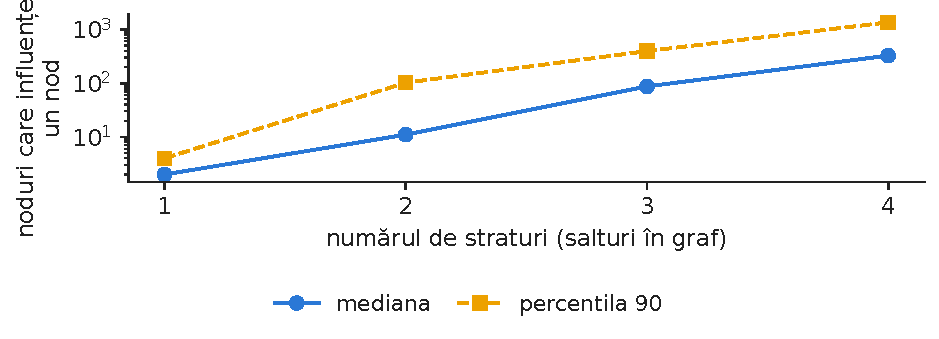
\includegraphics[width=\textwidth,height=0.406\textheight,keepaspectratio]{charts/ro/receptive_field.pdf}\end{center}\vspace{-3mm}
\chartsource{Sursa: Graful tranzacțiilor Bitcoin Elliptic (Weber et al., 2019). Date: graful tranzacțiilor Bitcoin Elliptic, 49 de pași de timp (circa două săptămîni fiecare).}
\vspace{0.5mm}
\begin{itemize}\setlength{\itemsep}{0pt}
  \item \textbf{Cîmpul receptiv} al unei tranzacții de test: mediana este 2 noduri după 1 strat, 11 după 2, 325 după 4
  \item \textbf{Coada}: percentila 90 ajunge la 1\,356 de noduri după 4 straturi
    \begin{itemize}\setlength{\itemsep}{0pt}
      \item Nodurile centrale leagă părți îndepărtate ale grafului
    \end{itemize}
\end{itemize}
\par\vfill\manager{$L$ straturi = $L$ salturi ale fluxului de bani
    \begin{itemize}\setlength{\itemsep}{0pt}
      \item Două salturi acoperă deja mare parte din ce ar verifica manual un investigator.
    \end{itemize}}\par\vspace{0.5mm}
\par\vfill\noindent{\scriptsize\color{FooterGray}(calcule proprii, 2.000 de noduri de test)}\hfill\qlink{NN\_L9\_receptive\_field}{Quantlets/L9/NN_L9_receptive_field}\par\vspace{0.5mm}
\end{frame}

\begin{frame}{Prea multe straturi fac toate nodurile să semene: suprasmoothing-ul (over-smoothing)}
\small
\begin{center}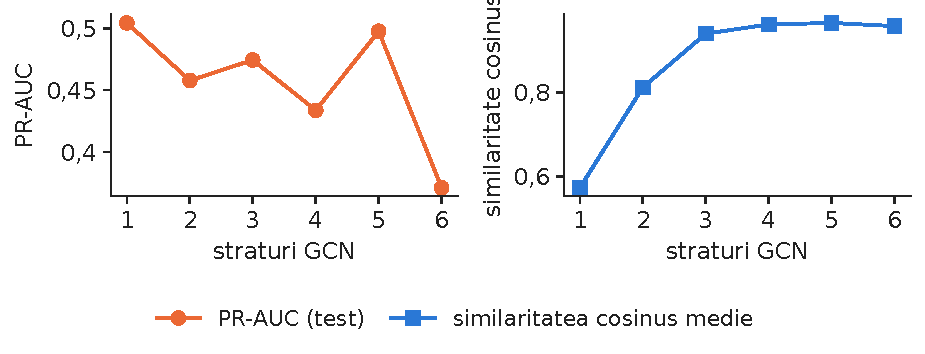
\includegraphics[width=\textwidth,height=0.336\textheight,keepaspectratio]{charts/ro/oversmoothing.pdf}\end{center}\vspace{-3mm}
\chartsource{Sursa: Graful tranzacțiilor Bitcoin Elliptic (Weber et al., 2019). Date: estimări proprii; antrenare pe pașii 1-34, pașii de timp de test 35-49.}
\vspace{0.5mm}
\begin{itemize}\setlength{\itemsep}{0pt}
  \item \textbf{Precizia}: PR-AUC 0{,}504 cu 1 strat GCN, 0{,}458 cu 2, 0{,}371 cu 6
    \begin{itemize}\setlength{\itemsep}{0pt}
      \item Adîncimea cea mai bună: 1
    \end{itemize}
  \item \textbf{Similaritatea}: similaritatea cosinus medie a reprezentărilor crește de la 0{,}57 (1 strat) la 0{,}96 (6 straturi)
    \begin{itemize}\setlength{\itemsep}{0pt}
      \item Medierea repetată le aduce spre un vector comun
    \end{itemize}
\end{itemize}
\par\vfill\manager{rețelele GNN sînt intenționat puțin adînci: două-trei straturi, apoi conexiuni reziduale dacă este nevoie de mai mult.}\par\vspace{0.5mm}
\par\vfill\noindent{\scriptsize\color{FooterGray}(calcule proprii, 2 semințe; Li, Han \& Wu, 2018)}\hfill\qlink{NN\_L9\_oversmoothing}{Quantlets/L9/NN_L9_oversmoothing}\par\vspace{0.5mm}
\end{frame}


\section{GCN, GraphSAGE și GAT}

\begin{frame}{GCN: media vecinilor ponderată cu gradele, apoi o regresie}
\footnotesize
\intuition{Un strat GCN este o regresie liniară pe media normalizată a nodului și a vecinilor lui, urmată de o unitate liniară rectificată (ReLU).}
\begin{columns}[T,onlytextwidth]
\begin{column}{0.53\textwidth}
\[ H^{(l+1)}=\ReLU\big(\hat A\,H^{(l)}W^{(l)}\big) \]\[ \mathbf h_v^{(l+1)}=\ReLU\Big(\sum_{u\in\mathcal N(v)\cup\{v\}}\frac{W^{(l)\top}\mathbf h_u^{(l)}}{\sqrt{\tilde d_u\tilde d_v}}\Big) \]{\footnotesize\begin{itemize}\setlength{\itemsep}{0pt}
  \item \textbf{\txtwhere}
    \begin{itemize}\setlength{\itemsep}{0pt}
      \item $H^{(l)}\in\R^{n\times d_l}$ = reprezentările nodurilor, $H^{(0)}=\mathbf X$
      \item $W^{(l)}$ = ponderi comune tuturor nodurilor
      \item $\ReLU(x)=\max(0,x)$
      \item Ieșirea: $\softmax(\hat A H^{(1)}W^{(2)})$.
    \end{itemize}
\end{itemize}\par}
\end{column}
\begin{column}{0.44\textwidth}
\begin{itemize}\setlength{\itemsep}{3pt}
  \item \textbf{Rețeaua GCN folosită}
    \begin{itemize}\setlength{\itemsep}{0pt}
      \item 2 straturi, 100 de unități ascunse, dropout 0,2: 26\,902 parametri
      \item Antrenare pe tot graful odată, 66 s pe sămînță, pe unitatea centrală de procesare (CPU)
    \end{itemize}
  \item \textbf{Costul}
    \begin{itemize}\setlength{\itemsep}{0pt}
      \item $O(|\mathcal E|\,d_l+n\,d_l d_{l+1})$ pe strat: liniar în numărul de muchii
    \end{itemize}
\end{itemize}
\end{column}
\end{columns}
\par\vfill\manager{o rețea GCN este analogul pe graf al unei medii mobile: robustă, ieftină și oarbă la care vecin contează cel mai mult.}\par\vspace{0.5mm}
\par\vfill\noindent{\scriptsize\color{FooterGray}(Kipf \& Welling, 2017)}\hfill\tryit{notebook, secțiunea 3}\par\vspace{0.5mm}
\end{frame}

\begin{frame}{GraphSAGE: separă nodul de vecini și eșantionează vecinii}
\footnotesize
\intuition{GraphSAGE alătură starea proprie a nodului și media unui eșantion de vecini, deci funcționează și pe noduri nevăzute la antrenare.}
\begin{columns}[T,onlytextwidth]
\begin{column}{0.53\textwidth}
\[ \mathbf h_v^{(l+1)}=\ReLU\Big(W_1^{(l)}\mathbf h_v^{(l)}+W_2^{(l)}\frac{1}{|\mathcal S(v)|}\sum_{u\in\mathcal S(v)}\mathbf h_u^{(l)}\Big) \]{\footnotesize\begin{itemize}\setlength{\itemsep}{0pt}
  \item \textbf{\txtwhere}
    \begin{itemize}\setlength{\itemsep}{0pt}
      \item $\mathcal S(v)\subseteq\mathcal N(v)$ = un eșantion aleator de cel mult $k$ vecini (toți, în rularea noastră pe tot graful)
      \item $W_1$, $W_2$ = ponderi separate pentru nod și pentru vecinătatea lui.
    \end{itemize}
\end{itemize}\par}
\end{column}
\begin{column}{0.44\textwidth}
\begin{itemize}\setlength{\itemsep}{3pt}
  \item \textbf{Inductiv}
    \begin{itemize}\setlength{\itemsep}{0pt}
      \item Ponderile nu depind de graf: tranzacțiile de mîine primesc un scor fără reantrenare
    \end{itemize}
  \item \textbf{Scalabil}
    \begin{itemize}\setlength{\itemsep}{0pt}
      \item Mini-loturi de eșantioane pe $k$ salturi: costul este limitat la $k^L$ pe nod, nu de gradul nodurilor centrale
    \end{itemize}
  \item \textbf{Pe Elliptic}
    \begin{itemize}\setlength{\itemsep}{0pt}
      \item F1 pe clasa ilicită 0{,}564 (abatere standard 0{,}022), PR-AUC 0{,}582
    \end{itemize}
\end{itemize}
\end{column}
\end{columns}
\par\vfill\manager{sistemele de plăți care dau scoruri în timp real au nevoie de straturi inductive precum GraphSAGE.}\par\vspace{0.5mm}
\par\vfill\noindent{\scriptsize\color{FooterGray}(Hamilton, Ying \& Leskovec, 2017)}\hfill\tryit{notebook, secțiunea 4}\par\vspace{0.5mm}
\end{frame}

\begin{frame}{GAT: rețeaua decide care vecin contează}
\footnotesize
\intuition{Un strat GAT ponderează fiecare vecin cu un scor învățat: atenția din cursul 7, restrînsă la muchii.}
\begin{columns}[T,onlytextwidth]
\begin{column}{0.56\textwidth}
\[ \alpha_{vu}=\frac{\exp\big(\mathrm{LeakyReLU}(\mathbf a^{\top}[W\mathbf h_v\,\|\,W\mathbf h_u])\big)}{\sum_{k\in\mathcal N(v)\cup\{v\}}\exp\big(\mathrm{LeakyReLU}(\mathbf a^{\top}[W\mathbf h_v\,\|\,W\mathbf h_k])\big)} \]\[ \mathbf h_v^{(l+1)}=\big\|_{k=1}^{K}\ \ReLU\Big(\sum_{u}\alpha_{vu}^{k}W^{k}\mathbf h_u\Big) \]{\footnotesize\begin{itemize}\setlength{\itemsep}{0pt}
  \item \textbf{\txtwhere}
    \begin{itemize}\setlength{\itemsep}{0pt}
      \item $\mathbf a$ = vectorul de atenție
      \item $\|$ = concatenare
      \item $K$ = numărul de capete (aici 4)
      \item Ponderile $\alpha_{vu}$ însumează unu pe vecinii lui $v$.
    \end{itemize}
\end{itemize}\par}
\end{column}
\begin{column}{0.41\textwidth}
\begin{itemize}\setlength{\itemsep}{3pt}
  \item \textbf{Legătura cu transformerele}
    \begin{itemize}\setlength{\itemsep}{0pt}
      \item Un transformer este o rețea GAT pe graful complet al tokenilor
    \end{itemize}
  \item \textbf{Pe Elliptic}
    \begin{itemize}\setlength{\itemsep}{0pt}
      \item 27\,302 parametri; F1 pe clasa ilicită 0{,}489, PR-AUC 0{,}496
    \end{itemize}
\end{itemize}
\end{column}
\end{columns}
\par\vfill\manager{ponderile de atenție sînt o primă explicație, nu una finală: arată unde s-a uitat modelul, nu de ce.}\par\vspace{0.5mm}
\par\vfill\noindent{\scriptsize\color{FooterGray}(Veličković et al., 2018)}\hfill\tryit{notebook, secțiunea 4}\par\vspace{0.5mm}
\end{frame}

\begin{frame}{Antrenarea pe un singur graf mare: măști, ponderi de clasă, oprire timpurie}
\footnotesize
\intuition{Toate nodurile transmit mesaje, dar în funcția de pierdere intră doar nodurile etichetate de antrenare; pașii de validare decid oprirea.}
\begin{columns}[T,onlytextwidth]
\begin{column}{0.53\textwidth}
\[ \loss(\btheta)=-\frac{1}{|\mathcal V_{tr}|}\sum_{v\in\mathcal V_{tr}}\big[w_1\,y_v\log\hat p_v+w_0(1-y_v)\log(1-\hat p_v)\big] \]{\footnotesize\begin{itemize}\setlength{\itemsep}{0pt}
  \item \textbf{\txtwhere}
    \begin{itemize}\setlength{\itemsep}{0pt}
      \item $\mathcal V_{tr}$ = nodurile etichetate din pașii 1--29
      \item $\hat p_v$ = probabilitatea estimată de ilicit
      \item $w_1=0{,}7$, $w_0=0{,}3$ = ponderile de clasă din Weber et al.\ (2019)
      \item Adam, rata de învățare 0,003, penalizarea ponderilor $5\cdot10^{-4}$.
    \end{itemize}
\end{itemize}\par}
\end{column}
\begin{column}{0.44\textwidth}
\begin{itemize}\setlength{\itemsep}{3pt}
  \item \textbf{Validarea}
    \begin{itemize}\setlength{\itemsep}{0pt}
      \item Nodurile etichetate din pașii 30--34: epoca cea mai bună după PR-AUC, răbdare 40 de epoci
      \item Epoca mediană reținută pentru GCN: 47
    \end{itemize}
  \item \textbf{Standardizare fără scurgeri de informație}
    \begin{itemize}\setlength{\itemsep}{0pt}
      \item Mediile și abaterile standard ale variabilelor numai din pașii 1--34
    \end{itemize}
\end{itemize}
\end{column}
\end{columns}
\par\vfill\manager{nodurile necunoscute nu se pierd: ele transmit mesaje între nodurile etichetate (învățare semi-supervizată).}\par\vspace{0.5mm}
\par\vfill\noindent{\scriptsize\color{FooterGray}(Kipf \& Welling, 2017; Weber et al., 2019)}\hfill\tryit{notebook, secțiunea 3}\par\vspace{0.5mm}
\end{frame}


\section{Studiu de caz: tranzacții Bitcoin ilicite}

\begin{frame}{Opt modele, un singur test în timp}
\footnotesize
{\scriptsize\renewcommand{\arraystretch}{1.05}\setlength{\tabcolsep}{4pt}
\begin{tabular}{@{}p{0.27\textwidth}p{0.66\textwidth}@{}}\toprule
Model & Ce vede \\ \midrule
Regresie logistică & doar variabilele locale (93), apoi toate cele 165 \\
Pădure aleatoare & toate variabilele; 100 de arbori, 50 de variabile la fiecare împărțire (Weber et al., 2019) \\
MLP (fără graf) & toate variabilele, aceleași straturi ca GCN, dar fără mesaje: izolează valoarea muchiilor \\
GCN, GraphSAGE, GAT & toate variabilele și graful; 2 straturi, 100 de unități \\
Pădure + GCN & toate variabilele și cele 100 de ieșiri ascunse GCN ale fiecărui nod \\
\bottomrule\end{tabular}}
\vspace{1mm}
\begin{itemize}\setlength{\itemsep}{2pt}
  \item \textbf{Măsuri pe pașii 35--49}: precizia, recall-ul și F1 pe clasa ilicită, la pragul 0,5
    \begin{itemize}\setlength{\itemsep}{0pt}
      \item PR-AUC (fără prag)
    \end{itemize}
  \item \textbf{Incertitudinea}: 3 semințe pentru fiecare rețea și pădure
    \begin{itemize}\setlength{\itemsep}{0pt}
      \item Bootstrap pe nodurile de test pentru diferențe
    \end{itemize}
\end{itemize}
\par\vfill\noindent{\scriptsize\color{FooterGray}(Weber et al., 2019)}\hfill\tryit{notebook, secțiunea 2}\par\vspace{0.5mm}
\end{frame}

\begin{frame}{Pe Elliptic pădurea conduce; straturile pe graf adaugă mai ales putere de ordonare unei rețele}
\small
\begin{center}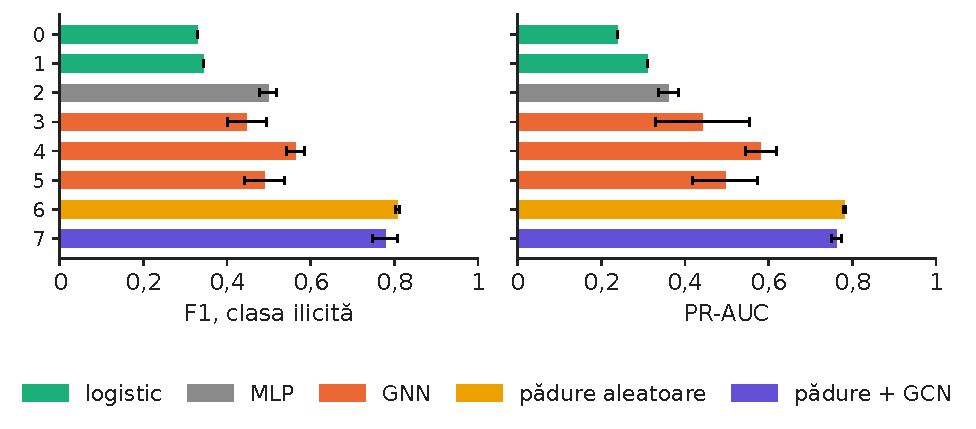
\includegraphics[width=\textwidth,height=0.520\textheight,keepaspectratio]{charts/ro/model_comparison.pdf}\end{center}\vspace{-3mm}
\chartsource{Sursa: Graful tranzacțiilor Bitcoin Elliptic (Weber et al., 2019). Date: estimări proprii; antrenare pe pașii 1-34, pașii de timp de test 35-49.}
\vspace{0.5mm}
\begin{itemize}\setlength{\itemsep}{0pt}
  \item \textbf{F1 pe clasa ilicită}: pădurea 0{,}808, pădurea + GCN 0{,}778, GCN 0{,}447, MLP 0{,}498, logistic 0{,}343
  \item \textbf{Valoarea muchiilor}: PR-AUC GCN minus MLP, cu aceleași straturi: \ensuremath{+}8{,}1 puncte
\end{itemize}
\par\vfill\noindent{\scriptsize\color{FooterGray}(calcule proprii; media $\pm$ abaterea standard pe 3 semințe)}\hfill\qlink{NN\_L9\_model\_comparison}{Quantlets/L9/NN_L9_model_comparison}\par\vspace{0.5mm}
\end{frame}

\begin{frame}{Precizie, recall și costul antrenării}
\footnotesize
\begin{columns}[T,onlytextwidth]
\begin{column}{0.56\textwidth}
{\scriptsize\renewcommand{\arraystretch}{1.05}\setlength{\tabcolsep}{4pt}
\begin{tabular}{@{}lrrrrr@{}}\toprule
Model & Prec. & Recall & F1 & PR-AUC & Sec. \\ \midrule
Logistic, locale & 0{,}208 & 0{,}789 & \cellcolor{Crimson!55}0{,}329 & \cellcolor{Crimson!55}0{,}239 & 0{,}8 \\
Logistic, toate & 0{,}220 & 0{,}771 & \cellcolor{Crimson!52}0{,}343 & \cellcolor{Crimson!40}0{,}311 & 1{,}8 \\
MLP & 0{,}517 & 0{,}483 & \cellcolor{Crimson!16}0{,}498 & \cellcolor{Crimson!30}0{,}361 & 59{,}2 \\
GCN & 0{,}484 & 0{,}494 & \cellcolor{Crimson!28}0{,}447 & \cellcolor{Crimson!14}0{,}442 & 65{,}5 \\
GraphSAGE & 0{,}569 & 0{,}561 & \cellcolor{Crimson!1}0{,}564 & \cellcolor{Forest!14}0{,}582 & 143{,}2 \\
GAT & 0{,}488 & 0{,}500 & \cellcolor{Crimson!18}0{,}489 & \cellcolor{Crimson!3}0{,}496 & 231{,}2 \\
Pădure aleatoare & 0{,}914 & 0{,}725 & \cellcolor{Forest!55}0{,}808 & \cellcolor{Forest!55}0{,}782 & 4{,}9 \\
Pădure + GCN & 0{,}933 & 0{,}668 & \cellcolor{Forest!48}0{,}778 & \cellcolor{Forest!51}0{,}763 & 186{,}0 \\
\bottomrule\end{tabular}}
\end{column}
\begin{column}{0.41\textwidth}
\begin{itemize}\setlength{\itemsep}{3pt}
  \item \textbf{Cum citim tabelul}
    \begin{itemize}\setlength{\itemsep}{0pt}
      \item Precizia = ponderea alertelor care sînt ilicite; recall = ponderea ilicitelor găsite
      \item Verde = cel mai bun, roșu = cel mai slab din coloană
    \end{itemize}
  \item \textbf{Pădurea}
    \begin{itemize}\setlength{\itemsep}{0pt}
      \item Precizie 0{,}914, recall 0{,}725
    \end{itemize}
  \item \textbf{Logistic, ponderi de clasă 0,3/0,7}
    \begin{itemize}\setlength{\itemsep}{0pt}
      \item Precizie 0{,}220, recall 0{,}771: ponderile cumpără recall cu alarme false
    \end{itemize}
\end{itemize}
\end{column}
\end{columns}
\par\vfill\manager{modelul potrivit depinde de costul unei erori: un caz de spălare ratat sau o oră pierdută de un analist.}\par\vspace{0.5mm}
\par\vfill\noindent{\scriptsize\color{FooterGray}(calcule proprii; sec.\ = timpul de antrenare pe sămînță, CPU)}\hfill\tryit{notebook, secțiunea 2}\par\vspace{0.5mm}
\end{frame}

\begin{frame}{Curbele precizie-recall: ordonarea din spatele lui F1}
\small
\begin{center}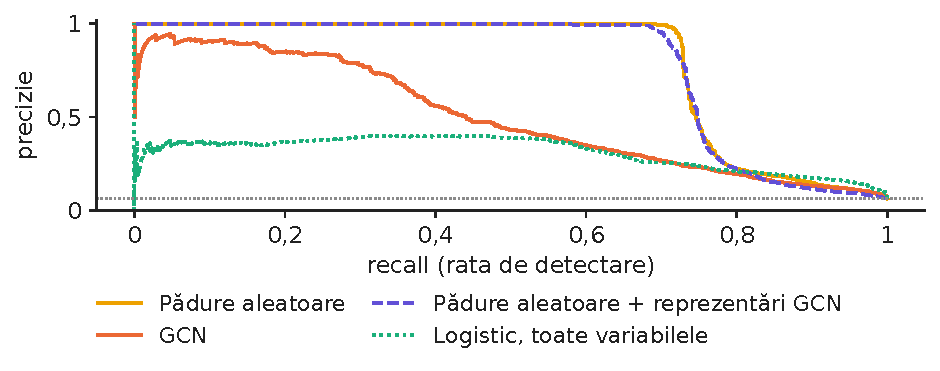
\includegraphics[width=\textwidth,height=0.580\textheight,keepaspectratio]{charts/ro/pr_curves.pdf}\end{center}\vspace{-3mm}
\chartsource{Sursa: Graful tranzacțiilor Bitcoin Elliptic (Weber et al., 2019). Date: estimări proprii; antrenare pe pașii 1-34, pașii de timp de test 35-49.}
\vspace{0.5mm}
\begin{itemize}\setlength{\itemsep}{0pt}
  \item \textbf{PR-AUC}: pădurea 0{,}782, pădurea + GCN 0{,}763, GCN 0{,}442, logistic 0{,}311
    \begin{itemize}\setlength{\itemsep}{0pt}
      \item Un scor aleator ar da 6{,}50\,\% (linia punctată)
    \end{itemize}
\end{itemize}
\par\vfill\noindent{\scriptsize\color{FooterGray}$\text{PR-AUC}=\sum_k (R_k-R_{k-1})P_k$}\hfill\qlink{NN\_L9\_pr\_curves}{Quantlets/L9/NN_L9_pr_curves}\par\vspace{0.5mm}
\end{frame}

\begin{frame}{Este diferența reală? Un bootstrap al tranzacțiilor de test}
\footnotesize
\intuition{Un singur set de test dă un singur număr; reeșantionarea nodurilor de test arată cît s-ar putea mișca acest număr.}
\begin{columns}[T,onlytextwidth]
\begin{column}{0.53\textwidth}
\[ \Delta^{*b}=\text{PR-AUC}_A\big(\mathcal T^{*b}\big)-\text{PR-AUC}_B\big(\mathcal T^{*b}\big),\quad b=1,\dots,B \]\[ \text{CI}_{95\%}=\big[q_{0.025}(\Delta^{*}),\ q_{0.975}(\Delta^{*})\big] \]{\footnotesize\begin{itemize}\setlength{\itemsep}{0pt}
  \item \textbf{\txtwhere}
    \begin{itemize}\setlength{\itemsep}{0pt}
      \item $\mathcal T^{*b}$ = noduri de test extrase cu întoarcere
      \item $B=1.000$
      \item Scorurile = media pe 3 semințe
      \item Aceeași extragere pentru ambele modele (comparație pereche).
    \end{itemize}
\end{itemize}\par}
\end{column}
\begin{column}{0.44\textwidth}
\begin{itemize}\setlength{\itemsep}{3pt}
  \item \textbf{Pădurea minus GCN}
    \begin{itemize}\setlength{\itemsep}{0pt}
      \item $\Delta$ = 0{,}285, intervalul de 95\,\% [0{,}259; 0{,}313]
    \end{itemize}
  \item \textbf{Pădurea + GCN minus pădurea}
    \begin{itemize}\setlength{\itemsep}{0pt}
      \item $\Delta$ = \ensuremath{-}0{,}008, intervalul de 95\,\% [\ensuremath{-}0{,}015; \ensuremath{-}0{,}002]
    \end{itemize}
  \item un interval care nu conține 0 susține o diferență reală pe această perioadă de test
\end{itemize}
\end{column}
\end{columns}
\par\vfill\manager{raportați intervalul, nu doar cîștigătorul: un comitet antifraudă decide pe intervale, nu pe a treia zecimală.}\par\vspace{0.5mm}
\par\vfill\noindent{\scriptsize\color{FooterGray}(Efron \& Tibshirani, 1993)}\hfill\tryit{notebook, secțiunea 2}\par\vspace{0.5mm}
\end{frame}

\begin{frame}{De ce pădurea este greu de bătut aici: variabilele ei transmit deja mesaje}
\footnotesize
\begin{columns}[T,onlytextwidth]
\begin{column}{0.49\textwidth}
\begin{itemize}\setlength{\itemsep}{4pt}
  \item \textbf{Transmitere de mesaje construită manual}
    \begin{itemize}\setlength{\itemsep}{0pt}
      \item 72 dintre cele 165 de variabile sînt agregate pe vecinii de la un salt (maxim, minim, abatere standard, corelație)
      \item Este un strat GNN fix, calculat de Elliptic înainte de publicarea datelor
    \end{itemize}
  \item \textbf{Doar variabilele locale}
    \begin{itemize}\setlength{\itemsep}{0pt}
      \item Regresia logistică are F1 0{,}329, față de 0{,}343 cu agregatele
    \end{itemize}
  \item \textbf{Arborii}
    \begin{itemize}\setlength{\itemsep}{0pt}
      \item Pragurile pe sume și numere se potrivesc tiparelor de fraudă care sînt reguli (``mai mult de $k$ intrări'')
    \end{itemize}
\end{itemize}
\end{column}
\begin{column}{0.48\textwidth}
\begin{itemize}\setlength{\itemsep}{4pt}
  \item \textbf{Unde își justifică rețelele GNN costul}
    \begin{itemize}\setlength{\itemsep}{0pt}
      \item Grafuri brute, fără agregate construite manual
      \item Tipare pe mai multe salturi (stratificarea prin multe conturi)
      \item Scoruri inductive pentru noduri noi și reprezentări pentru alte modele
    \end{itemize}
  \item \textbf{Combinați}
    \begin{itemize}\setlength{\itemsep}{0pt}
      \item Pădure + reprezentări GCN: variația lui F1 este \ensuremath{-}3{,}0 puncte
    \end{itemize}
\end{itemize}
\end{column}
\end{columns}
\par\vfill\manager{înainte de a antrena o rețea GNN, verificați dacă furnizorul datelor nu a agregat deja vecinătatea.}\par\vspace{0.5mm}
\par\vfill\noindent{\scriptsize\color{FooterGray}(Weber et al., 2019)}\hfill\tryit{notebook, secțiunea 2}\par\vspace{0.5mm}
\end{frame}

\begin{frame}{Închiderea unei piețe ilegale strică toate modelele: schimbarea conceptului}
\small
\begin{center}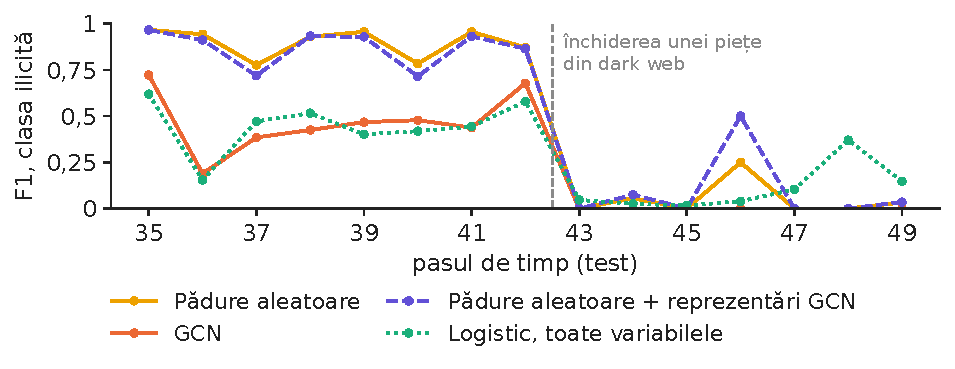
\includegraphics[width=\textwidth,height=0.373\textheight,keepaspectratio]{charts/ro/f1_by_timestep.pdf}\end{center}\vspace{-3mm}
\chartsource{Sursa: Graful tranzacțiilor Bitcoin Elliptic (Weber et al., 2019). Date: estimări proprii; antrenare pe pașii 1-34, pașii de timp de test 35-49.}
\vspace{0.5mm}
\begin{itemize}\setlength{\itemsep}{0pt}
  \item \textbf{Înainte de pasul 43}: F1 mediu pădure 0{,}898, GCN 0{,}473
    \begin{itemize}\setlength{\itemsep}{0pt}
      \item \textbf{de la pasul 43}: 0{,}048 și 0{,}000
    \end{itemize}
  \item \textbf{Comportament nou}: după închiderea unei piețe ilegale importante, fluxurile ilicite și-au schimbat forma
    \begin{itemize}\setlength{\itemsep}{0pt}
      \item Niciun model antrenat pe pașii 1--34 nu o văzuse (Weber et al., 2019)
    \end{itemize}
\end{itemize}
\par\vfill\manager{monitorizați F1 pe fiecare perioadă și reantrenați pe etichete recente
    \begin{itemize}\setlength{\itemsep}{0pt}
      \item Un model AML static îmbătrînește în cîteva săptămîni.
    \end{itemize}}\par\vspace{0.5mm}
\par\vfill\noindent{\scriptsize\color{FooterGray}}\hfill\qlink{NN\_L9\_f1\_by\_timestep}{Quantlets/L9/NN_L9_f1_by_timestep}\par\vspace{0.5mm}
\end{frame}

\begin{frame}{Ce obține o echipă de investigații din 1\,000 de alerte}
\small
\begin{center}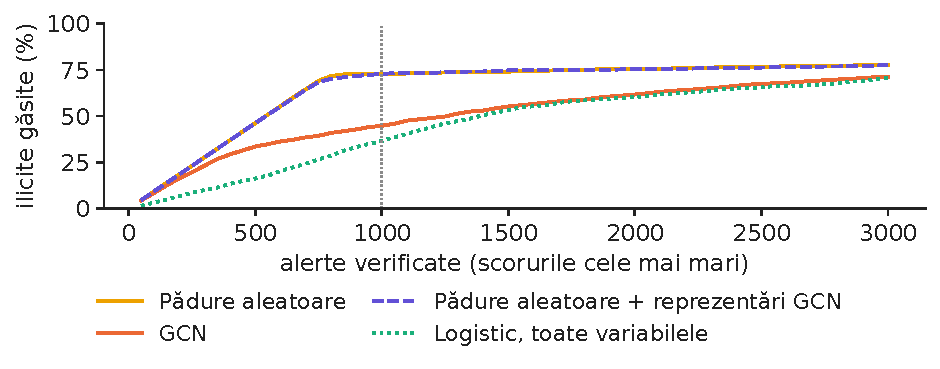
\includegraphics[width=\textwidth,height=0.402\textheight,keepaspectratio]{charts/ro/alert_budget.pdf}\end{center}\vspace{-3mm}
\chartsource{Sursa: Graful tranzacțiilor Bitcoin Elliptic (Weber et al., 2019). Date: estimări proprii; antrenare pe pașii 1-34, pașii de timp de test 35-49.}
\vspace{0.5mm}
\begin{itemize}\setlength{\itemsep}{0pt}
  \item \textbf{Primele 1\,000 de scoruri} din perioada de test conțin 72{,}9\,\% dintre toate tranzacțiile ilicite pentru pădure, 44{,}8\,\% pentru GCN și 72{,}9\,\% pentru pădure + GCN
  \item \textbf{Rata de reușită} a acestor alerte: 78{,}9\,\% (pădurea), 48{,}5\,\% (GCN), din 1\,083 de tranzacții ilicite de test
\end{itemize}
\par\vfill\manager{dimensionați echipa după această curbă: bugetul de alerte, nu F1, este constrîngerea unui departament de conformitate.}\par\vspace{0.5mm}
\par\vfill\noindent{\scriptsize\color{FooterGray}}\hfill\qlink{NN\_L9\_alert\_budget}{Quantlets/L9/NN_L9_alert_budget}\par\vspace{0.5mm}
\end{frame}

\begin{frame}{Rețeaua GCN învață un spațiu în care tranzacțiile ilicite se adună}
\small
\begin{center}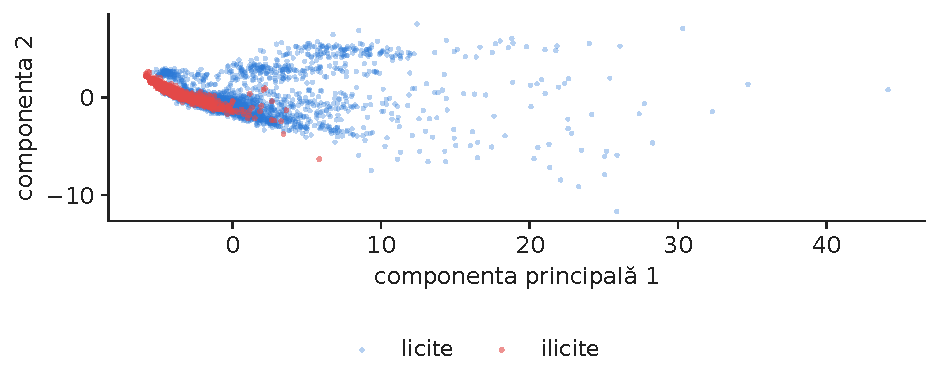
\includegraphics[width=\textwidth,height=0.532\textheight,keepaspectratio]{charts/ro/gcn_embeddings.pdf}\end{center}\vspace{-3mm}
\chartsource{Sursa: Graful tranzacțiilor Bitcoin Elliptic (Weber et al., 2019). Date: estimări proprii; antrenare pe pașii 1-34, pașii de timp de test 35-49.}
\vspace{0.5mm}
\begin{itemize}\setlength{\itemsep}{0pt}
  \item \textbf{Stratul ascuns} al rețelei GCN (100 de dimensiuni), proiectat prin analiza componentelor principale (PCA) pe primele două componente: 79{,}2\,\% din varianță
  \item \textbf{Refolosire}: acești vectori sînt intrările modelului pădure + GCN și pot alimenta orice alt model de risc
\end{itemize}
\par\vfill\noindent{\scriptsize\color{FooterGray}(calcule proprii; 1\,083 de noduri ilicite și 3.000 de noduri licite de test)}\hfill\qlink{NN\_L9\_gcn\_embeddings}{Quantlets/L9/NN_L9_gcn_embeddings}\par\vspace{0.5mm}
\end{frame}

\begin{frame}{Adăugarea variabilelor de graf reordonează explicațiile}
\small
\begin{center}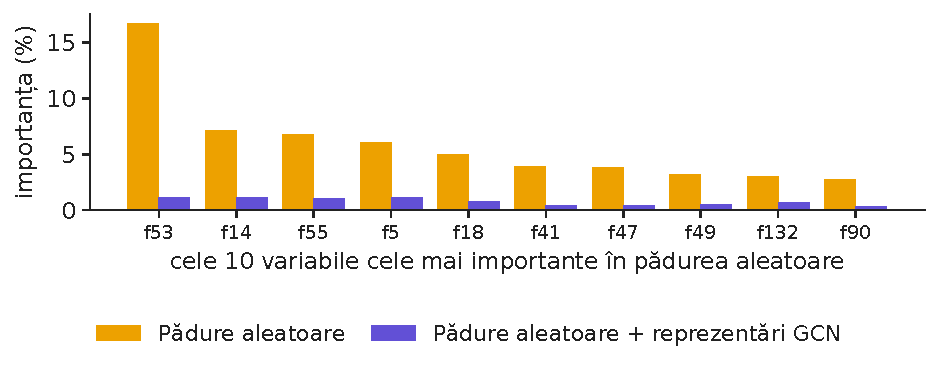
\includegraphics[width=\textwidth,height=0.367\textheight,keepaspectratio]{charts/ro/importance_shift.pdf}\end{center}\vspace{-3mm}
\chartsource{Sursa: Graful tranzacțiilor Bitcoin Elliptic (Weber et al., 2019). Date: estimări proprii; antrenare pe pașii 1-34, pașii de timp de test 35-49.}
\vspace{0.5mm}
\begin{itemize}\setlength{\itemsep}{0pt}
  \item \textbf{Masa importanței}: primele 10 variabile ale pădurii au 58{,}2\,\% din importanță
    \begin{itemize}\setlength{\itemsep}{0pt}
      \item Cu reprezentările GCN păstrează 7{,}4\,\%, reprezentările iau 73{,}9\,\%
    \end{itemize}
  \item \textbf{Stabilitatea pe 3 reantrenări}: corelația Spearman medie a importanțelor 0{,}973 (pădurea) și 0{,}896 (pădure + GCN)
\end{itemize}
\par\vfill\manager{comparați explicațiile între reantrenări înainte de a interpreta o schimbare de model ca o schimbare de explicație.}\par\vspace{0.5mm}
\par\vfill\noindent{\scriptsize\color{FooterGray}}\hfill\qlink{NN\_L9\_importance\_shift}{Quantlets/L9/NN_L9_importance_shift}\par\vspace{0.5mm}
\end{frame}


\section{Rețelele GNN în producție}

\begin{frame}{Patru capcane ale modelelor pe graf în finanțe}
\footnotesize
\begin{columns}[T,onlytextwidth]
\begin{column}{0.49\textwidth}
\begin{itemize}\setlength{\itemsep}{5pt}
  \item \textbf{Scurgeri de informație prin muchii}
    \begin{itemize}\setlength{\itemsep}{0pt}
      \item Un nod de test nu trebuie să primească mesaje din viitor
      \item În Elliptic 100{,}0\,\% dintre muchii rămîn în același pas de timp, deci împărțirea în timp este curată
    \end{itemize}
  \item \textbf{Puține etichete}
    \begin{itemize}\setlength{\itemsep}{0pt}
      \item Doar 22{,}9\,\% dintre noduri sînt etichetate; etichetele vin din investigații anterioare și favorizează cazurile deja găsite
    \end{itemize}
\end{itemize}
\end{column}
\begin{column}{0.48\textwidth}
\begin{itemize}\setlength{\itemsep}{5pt}
  \item \textbf{Schimbarea în timp}
    \begin{itemize}\setlength{\itemsep}{0pt}
      \item Infractorii se adaptează: închiderea din pasul 43 a schimbat tiparele
      \item Rețelele GNN temporale (EvolveGCN) lasă ponderile să evolueze în timp
    \end{itemize}
  \item \textbf{Explicabilitatea}
    \begin{itemize}\setlength{\itemsep}{0pt}
      \item Un raport de activitate suspectă are nevoie de o justificare pe care un supraveghetor o poate citi
      \item GNNExplainer găsește subgraful și variabilele din spatele unei predicții
    \end{itemize}
\end{itemize}
\end{column}
\end{columns}
\par\vfill\manager{testați un model pe graf așa cum va funcționa: pe perioade ulterioare, cu etichetele disponibile atunci.}\par\vspace{0.5mm}
\par\vfill\noindent{\scriptsize\color{FooterGray}(Pareja et al., 2020; Ying et al., 2019)}\par\vspace{0.5mm}
\end{frame}

\begin{frame}{Grafuri peste tot în finanțe}
\footnotesize
\begin{columns}[T,onlytextwidth]
\begin{column}{0.49\textwidth}
\begin{itemize}\setlength{\itemsep}{5pt}
  \item \textbf{Plăți și carduri}
    \begin{itemize}\setlength{\itemsep}{0pt}
      \item Grafuri deținător--comerciant: un terminal compromis leagă multe victime
    \end{itemize}
  \item \textbf{Credit}
    \begin{itemize}\setlength{\itemsep}{0pt}
      \item Rețele de garanți și furnizori: neplata se propagă prin creditul comercial
    \end{itemize}
  \item \textbf{Cripto}
    \begin{itemize}\setlength{\itemsep}{0pt}
      \item Grafuri de adrese și tranzacții (acest curs), detectarea serviciilor de amestecare, gruparea portofelelor
    \end{itemize}
\end{itemize}
\end{column}
\begin{column}{0.48\textwidth}
\begin{itemize}\setlength{\itemsep}{5pt}
  \item \textbf{Risc sistemic}
    \begin{itemize}\setlength{\itemsep}{0pt}
      \item Expuneri interbancare și rețele de dependență în cozi: cine cade dacă o bancă cade
    \end{itemize}
  \item \textbf{Piețe}
    \begin{itemize}\setlength{\itemsep}{0pt}
      \item Grafuri de acțiuni legate prin corelație, lanț de aprovizionare sau acționariat, pentru prognoza randamentelor
    \end{itemize}
  \item \textbf{Energie}
    \begin{itemize}\setlength{\itemsep}{0pt}
      \item Rețelele electrice și zonele de preț interconectate sînt grafuri prin construcție
    \end{itemize}
\end{itemize}
\end{column}
\end{columns}
\par\vfill\manager{ori de cîte ori riscul unei unități depinde de contrapărțile ei, un model pe graf merită încercat.}\par\vspace{0.5mm}
\par\vfill\noindent{\scriptsize\color{FooterGray}(Hamilton, 2020; Bishop \& Bishop, 2024, ch.\ 13)}\par\vspace{0.5mm}
\end{frame}


\section{Concluzii}

\begin{frame}{Ce reținem}
\small
\begin{itemize}\setlength{\itemsep}{6pt}
  \item \textbf{Un strat GNN} = mesaj, agregare care nu depinde de ordine, actualizare
    \begin{itemize}\setlength{\itemsep}{0pt}
      \item GCN face media cu ponderi după grad, GraphSAGE separă nodul de vecini, GAT învață ponderile
    \end{itemize}
  \item \textbf{Adîncimea} = numărul de salturi: două straturi ajung la o mediană de 11 tranzacții
    \begin{itemize}\setlength{\itemsep}{0pt}
      \item Mai multe straturi netezesc excesiv (PR-AUC 0{,}371 cu 6 straturi)
    \end{itemize}
  \item \textbf{Pe Elliptic} muchiile ajută o rețea (GCN față de MLP: \ensuremath{+}8{,}1 puncte PR-AUC), dar o pădure aleatoare pe variabile deja agregate conduce (F1 0{,}808)
  \item \textbf{Judecați modelele AML} pe perioade ulterioare, cu PR-AUC, bugete de alerte și intervale bootstrap
    \begin{itemize}\setlength{\itemsep}{0pt}
      \item Urmăriți schimbarea în timp și stabilitatea explicațiilor
    \end{itemize}
\end{itemize}
\end{frame}

\begin{frame}{Cercetările grupului nostru: grafuri, fraudă și explicații}
\footnotesize
\begin{itemize}\setlength{\itemsep}{5pt}
  \item \textbf{Stabilitatea explicațiilor în detectarea fraudei cu variabile de graf} (Diaconu \& Pele, 2026)
    \begin{itemize}\setlength{\itemsep}{0pt}
      \item Lucrarea tratează reantrenarea completă a modelului drept unitate de inferență și compară explicațiile SHapley Additive exPlanations (SHAP) ale modelelor de fraudă cu și fără reprezentări de graf, față de controale fără graf, cu aceeași dimensiune și covarianță
    \end{itemize}
  \item \textbf{Rezultate}: adăugarea de variabile poate micșora mecanic atribuirile variabilelor originale
    \begin{itemize}\setlength{\itemsep}{0pt}
      \item După ce se ține cont de variabilitatea reantrenării, controalele fără graf reproduc cea mai mare parte a variației stabilității SHAP marginale, iar ordonările locale, la nivel de rînd, se schimbă
    \end{itemize}
  \item \textbf{Energy Financial Risk Meter} (Toma, Dima, Grecu, Pele \& Lessmann, 2026): măsoară riscul sistemic din sectorul energetic al Uniunii Europene pe baza rețelei de dependențe în cozi dintre firme
\end{itemize}
\vspace{1mm}{\scriptsize Rezultatele de pe acest slide sînt cele din lucrări; cifrele de pe celelalte slide-uri provin din calculele noastre.}
\par\vfill\noindent{\scriptsize\color{FooterGray}(Academia de Studii Economice din București; Academia Română, Institutul de Prognoză Economică)}\par\vspace{0.5mm}
\end{frame}

\begin{frame}{Lecturi și resurse suplimentare}
\small
\begin{columns}[T,onlytextwidth]
\begin{column}{0.52\textwidth}
\begin{itemize}\setlength{\itemsep}{4pt}
  \item \textbf{Bishop \& Bishop (2024)}, capitolul 13: rețele neuronale pe grafuri, de la transmiterea mesajelor la atenția pe graf
  \item \textbf{Hamilton (2020)}, \textit{Graph Representation Learning}, versiune gratuită: \href{https://www.cs.mcgill.ca/~wlh/grl_book/}{cs.mcgill.ca/\textasciitilde wlh/grl\_book}.
  \item \textbf{PyTorch Geometric}, tutoriale: \href{https://pytorch-geometric.readthedocs.io}{pytorch-geometric.readthedocs.io}.
\end{itemize}
\end{column}
\begin{column}{0.45\textwidth}
\begin{itemize}\setlength{\itemsep}{4pt}
  \item \textbf{Setul Elliptic} și lucrarea originală: \href{https://arxiv.org/abs/1908.02591}{arXiv:1908.02591}.
  \item \textbf{Acest curs}: cod, date, notebook-uri --- \href{https://github.com/danpele/NEURAL_BIZ}{github.com/danpele/NEURAL\_BIZ}.
  \item \textbf{Exercițiu practic}: notebook-ul reproduce toate graficele și cifrele acestui curs
\end{itemize}
\end{column}
\end{columns}
\end{frame}

\begin{frame}{Test 1: permutări}
\small
\begin{itemize}
  \item Renumerotăm tranzacțiile grafului.
    \begin{itemize}\setlength{\itemsep}{0pt}
      \item Ce trebuie să se întîmple cu scorurile GCN?
    \end{itemize}
\end{itemize}
\vspace{2mm}
\begin{exampleblock}{R\u{a}spuns}
\begin{itemize}
  \item Se permută la fel și altfel nu se schimbă: un strat GNN este echivariant la permutări, pentru că agregarea pe vecini nu depinde de ordine
\end{itemize}
\end{exampleblock}
\end{frame}

\begin{frame}{Test 2: adîncimea}
\small
\begin{itemize}
  \item De ce nu folosim zece straturi GCN, ca să vedem zece salturi ale fluxului de bani?
\end{itemize}
\vspace{2mm}
\begin{exampleblock}{R\u{a}spuns}
\begin{itemize}
  \item Medierea repetată face toate reprezentările asemănătoare (over-smoothing): pe Elliptic, PR-AUC scade de la 0{,}458 (2 straturi) la 0{,}371 (6 straturi)
\end{itemize}
\end{exampleblock}
\end{frame}

\begin{frame}{Test 3: modelul de referință puternic}
\small
\begin{itemize}
  \item De ce pădurea aleatoare fără graf bate rețeaua GCN pe Elliptic?
\end{itemize}
\vspace{2mm}
\begin{exampleblock}{R\u{a}spuns}
\begin{itemize}
  \item 72 dintre variabile sînt deja agregate pe vecini, un strat de transmitere a mesajelor construit manual
    \begin{itemize}\setlength{\itemsep}{0pt}
      \item În plus, arborii prind bine pragurile de tip regulă ale fraudei
    \end{itemize}
\end{itemize}
\end{exampleblock}
\end{frame}

\begin{frame}{Test 4: evaluarea}
\small
\begin{itemize}
  \item Doar 6{,}50\,\% dintre tranzacțiile de test sînt ilicite.
    \begin{itemize}\setlength{\itemsep}{0pt}
      \item Ce măsură l-ar induce în eroare pe un ofițer de conformitate?
    \end{itemize}
\end{itemize}
\vspace{2mm}
\begin{exampleblock}{R\u{a}spuns}
\begin{itemize}
  \item Acuratețea: dacă etichetăm totul ca licit avem dreptate în majoritatea cazurilor și nu găsim niciun infractor
    \begin{itemize}\setlength{\itemsep}{0pt}
      \item Folosim precizia, recall-ul, PR-AUC și bugetul de alerte
    \end{itemize}
\end{itemize}
\end{exampleblock}
\end{frame}

\begin{frame}{Test 5: atenția pe grafuri}
\small
\begin{itemize}
  \item Care este legătura dintre un strat GAT și transformerul din cursul 7?
\end{itemize}
\vspace{2mm}
\begin{exampleblock}{R\u{a}spuns}
\begin{itemize}
  \item Ambele ponderează vecinii cu un softmax al unor scoruri învățate
    \begin{itemize}\setlength{\itemsep}{0pt}
      \item Transformerul aplică atenția pe graful complet al tokenilor, GAT o restrînge la muchiile grafului
    \end{itemize}
\end{itemize}
\end{exampleblock}
\end{frame}

\begin{frame}{Bibliografie (1/2)}
\scriptsize
\begin{itemize}\setlength{\itemsep}{0pt}\scriptsize
\item Bishop, C.\,M.\ \& Bishop, H.\ (2024). \textit{Deep Learning: Foundations and Concepts}, ch.\ 13. Springer. \href{https://doi.org/10.1007/978-3-031-45468-4}{doi:10.1007/978-3-031-45468-4}
\item Breiman, L.\ (2001). Random forests. \textit{Machine Learning}, 45(1), 5--32. \href{https://doi.org/10.1023/A:1010933404324}{doi:10.1023/A:1010933404324}
\item Diaconu, D.\ \& Pele, D.\,T.\ (2026). Testing SHAP stability under distribution shift in graph-enhanced fraud detection. Submitted to \textit{Expert Systems with Applications}. Code: \href{https://github.com/QuantLet/GNN_XAI_Stability}{github.com/QuantLet/GNN\_XAI\_Stability}
\item Efron, B.\ \& Tibshirani, R.\,J.\ (1993). \textit{An Introduction to the Bootstrap}. Chapman \& Hall. \href{https://doi.org/10.1201/9780429246593}{doi:10.1201/9780429246593}
\item Fey, M.\ \& Lenssen, J.\,E.\ (2019). Fast graph representation learning with PyTorch Geometric. ICLR Workshop on Representation Learning on Graphs and Manifolds. \href{https://arxiv.org/abs/1903.02428}{arXiv:1903.02428}
\item Gilmer, J., Schoenholz, S.\,S., Riley, P.\,F., Vinyals, O.\ \& Dahl, G.\,E.\ (2017). Neural message passing for quantum chemistry. \textit{Proceedings of ICML}, PMLR 70, 1263--1272. \href{https://arxiv.org/abs/1704.01212}{arXiv:1704.01212}
\item Hamilton, W.\,L., Ying, R.\ \& Leskovec, J.\ (2017). Inductive representation learning on large graphs. \textit{Advances in Neural Information Processing Systems}, 30. \href{https://arxiv.org/abs/1706.02216}{arXiv:1706.02216}
\item Hamilton, W.\,L.\ (2020). \textit{Graph Representation Learning}. Morgan \& Claypool. \href{https://doi.org/10.2200/S01045ED1V01Y202009AIM046}{doi:10.2200/S01045ED1V01Y202009AIM046}
\item Kipf, T.\,N.\ \& Welling, M.\ (2017). Semi-supervised classification with graph convolutional networks. \textit{International Conference on Learning Representations}. \href{https://arxiv.org/abs/1609.02907}{arXiv:1609.02907}
\end{itemize}
\end{frame}

\begin{frame}{Bibliografie (2/2)}
\scriptsize
\begin{itemize}\setlength{\itemsep}{0pt}\scriptsize
\item Li, Q., Han, Z.\ \& Wu, X.-M.\ (2018). Deeper insights into graph convolutional networks for semi-supervised learning. \textit{Proceedings of the AAAI Conference on Artificial Intelligence}, 32(1). \href{https://doi.org/10.1609/aaai.v32i1.11604}{doi:10.1609/aaai.v32i1.11604}
\item Lundberg, S.\,M.\ \& Lee, S.-I.\ (2017). A unified approach to interpreting model predictions. \textit{Advances in Neural Information Processing Systems}, 30. \href{https://arxiv.org/abs/1705.07874}{arXiv:1705.07874}
\item Pareja, A., Domeniconi, G., Chen, J.\ et al.\ (2020). EvolveGCN: Evolving graph convolutional networks for dynamic graphs. \textit{Proceedings of the AAAI Conference on Artificial Intelligence}, 34(4), 5363--5370. \href{https://doi.org/10.1609/aaai.v34i04.5984}{doi:10.1609/aaai.v34i04.5984}
\item Toma, F.-M., Dima, D.-M., Grecu, R., Pele, D.\,T.\ \& Lessmann, S.\ (2026). Energy Financial Risk Meter: Systemic risk in the EU energy sector. SSRN Working Paper 6985301. \href{https://doi.org/10.2139/ssrn.6985301}{doi:10.2139/ssrn.6985301}
\item Veličković, P., Cucurull, G., Casanova, A., Romero, A., Liò, P.\ \& Bengio, Y.\ (2018). Graph attention networks. \textit{International Conference on Learning Representations}. \href{https://arxiv.org/abs/1710.10903}{arXiv:1710.10903}
\item Weber, M., Domeniconi, G., Chen, J., Weidele, D.\,K.\,I., Bellei, C., Robinson, T.\ \& Leiserson, C.\,E.\ (2019). Anti-money laundering in Bitcoin: Experimenting with graph convolutional networks for financial forensics. KDD Workshop on Anomaly Detection in Finance. \href{https://arxiv.org/abs/1908.02591}{arXiv:1908.02591}
\item Xu, K., Hu, W., Leskovec, J.\ \& Jegelka, S.\ (2019). How powerful are graph neural networks? \textit{International Conference on Learning Representations}. \href{https://arxiv.org/abs/1810.00826}{arXiv:1810.00826}
\item Ying, R., Bourgeois, D., You, J., Zitnik, M.\ \& Leskovec, J.\ (2019). GNNExplainer: Generating explanations for graph neural networks. \textit{Advances in Neural Information Processing Systems}, 32. \href{https://arxiv.org/abs/1903.03894}{arXiv:1903.03894}
\end{itemize}
\end{frame}

\appendix

\section*{Anexă}

\begin{frame}{Anexa A: de la filtrele spectrale la stratul GCN}
\small
\begin{columns}[T,onlytextwidth]
\begin{column}{0.52\textwidth}
\[ g_\theta\star\mathbf x\approx\sum_{k=0}^{K}\theta_k T_k(\tilde L)\,\mathbf x,\quad \tilde L=\tfrac{2}{\lambda_{\max}}L_{sym}-I \]\[ K=1,\ \lambda_{\max}\approx2:\quad g_\theta\star\mathbf x\approx\theta_0\mathbf x-\theta_1D^{-1/2}AD^{-1/2}\mathbf x \]\[ \theta=\theta_0=-\theta_1:\quad \theta\,(I+D^{-1/2}AD^{-1/2})\,\mathbf x\ \to\ \theta\,\hat A\,\mathbf x \]
\end{column}
\begin{column}{0.45\textwidth}
\begin{itemize}\setlength{\itemsep}{3pt}
  \item $T_k$ = polinoamele Cebîșev
    \begin{itemize}\setlength{\itemsep}{0pt}
      \item $L_{sym}=I-D^{-1/2}AD^{-1/2}$
      \item Un polinom de grad $K$ amestecă doar noduri aflate la cel mult $K$ salturi
    \end{itemize}
  \item Un singur parametru comun evită supraînvățarea
    \begin{itemize}\setlength{\itemsep}{0pt}
      \item Trucul de renormalizare $I+D^{-1/2}AD^{-1/2}\to\tilde D^{-1/2}\tilde A\tilde D^{-1/2}$ ține valorile proprii în $(-1,1]$
    \end{itemize}
  \item Cu $d$ variabile de intrare și $d'$ ieșiri, $\theta$ devine matricea $W\in\R^{d\times d'}$
\end{itemize}
\end{column}
\end{columns}
\par\vfill\noindent{\scriptsize\color{FooterGray}(Kipf \& Welling, 2017)}\par\vspace{0.5mm}
\end{frame}

\begin{frame}{Anexa B: testul Weisfeiler--Leman}
\small
\begin{columns}[T,onlytextwidth]
\begin{column}{0.50\textwidth}
\[ c_v^{(l+1)}=\operatorname{hash}\Big(c_v^{(l)},\ \{\!\{c_u^{(l)}:u\in\mathcal N(v)\}\!\}\Big) \]
\end{column}
\begin{column}{0.47\textwidth}
\begin{itemize}\setlength{\itemsep}{3pt}
  \item Se pornește cu aceeași culoare pentru toate nodurile
    \begin{itemize}\setlength{\itemsep}{0pt}
      \item Se rafinează prin aplicarea unei funcții hash culorii nodului și multisetului de culori ale vecinilor
    \end{itemize}
  \item Două grafuri cu histograme de culori diferite nu sînt izomorfe
    \begin{itemize}\setlength{\itemsep}{0pt}
      \item Histogramele egale nu decid
    \end{itemize}
  \item O rețea GNN cu transmitere de mesaje deosebește cel mult cît testul WL
    \begin{itemize}\setlength{\itemsep}{0pt}
      \item GIN atinge această limită cu agregare prin sumă și o actualizare injectivă
    \end{itemize}
\end{itemize}
\end{column}
\end{columns}
\par\vfill\noindent{\scriptsize\color{FooterGray}(Xu et al., 2019)}\par\vspace{0.5mm}
\end{frame}

\begin{frame}{Anexa C: setările experimentului}
\small
{\scriptsize\renewcommand{\arraystretch}{1.05}\setlength{\tabcolsep}{4pt}
\begin{tabular}{@{}p{0.30\textwidth}p{0.62\textwidth}@{}}\toprule
Setare & Valoare \\ \midrule
Împărțirea & antrenare pașii 1--29, validare 30--34, test 35--49 (numai nodurile etichetate intră în funcția de pierdere) \\
Rețele & 2 straturi, 100 de unități, ReLU, dropout 0,2; GAT: 4 capete a cîte 25; Adam, rata 0,003, penalizare $5\cdot10^{-4}$; cel mult 300 de epoci, răbdare 40 \\
Ponderi de clasă & 0,3 / 0,7 \\
Pădure aleatoare & 100 de arbori, 50 de variabile la fiecare împărțire, variabile nestandardizate \\
Semințe & 1, 2, 3 \\
Programe, echipament & PyTorch, PyTorch Geometric, scikit-learn; procesorul unui laptop, în total 0{,}1 minute \\
\bottomrule\end{tabular}}
\par\vfill\noindent{\scriptsize\color{FooterGray}(Weber et al., 2019; Fey \& Lenssen, 2019)}\par\vspace{0.5mm}
\end{frame}

\end{document}
